\documentclass{book}

\usepackage{indentfirst}
\usepackage{booktabs}
\usepackage{multirow}
\usepackage{framed}
\usepackage{graphicx}
\usepackage{float}


\begin{document}


\title{EE101 Final Project Report \\ Team 32}
\author{ Litao Zhou, Shaoheng Fang, Shiwen Dong, Hongbo Yang}

\date{\today}




\maketitle


\tableofcontents


\frontmatter

\chapter {Preface}

\section* {Who we are}

We are a group of freshman students at SJTU working for the 2019 Spring EE101 course final project. We are heading for a website which allows users to search for papers and learn more about the details from our webpage and visualized charts. Our website is a local one based on a local MySQL database and a local solr search engine. The programming and coding languages we've used in this project involves Python, PHP, javascript, HTML and CSS.

\section* {What we have}


Start from the index page, by typing the keywords you want to search about, you can access the search page. And then you can jump between all the information pages as you will. 

Based on the type of data and the way we present them, the contents of our web fall into 5 parts, namely search (result), papers, authors, affiliations and conferences. Every section is made up of several subpages demonstrating different functions. The main functions and features of every section are listed as follows. The name behind every row represents the person who mainly takes charge, but it should be decleared that all the team members have been helping address each other's probelms all the way through the project, and must have somehow contributed to the part that he is not in charge of.

\begin{figure}[htp]
\centering
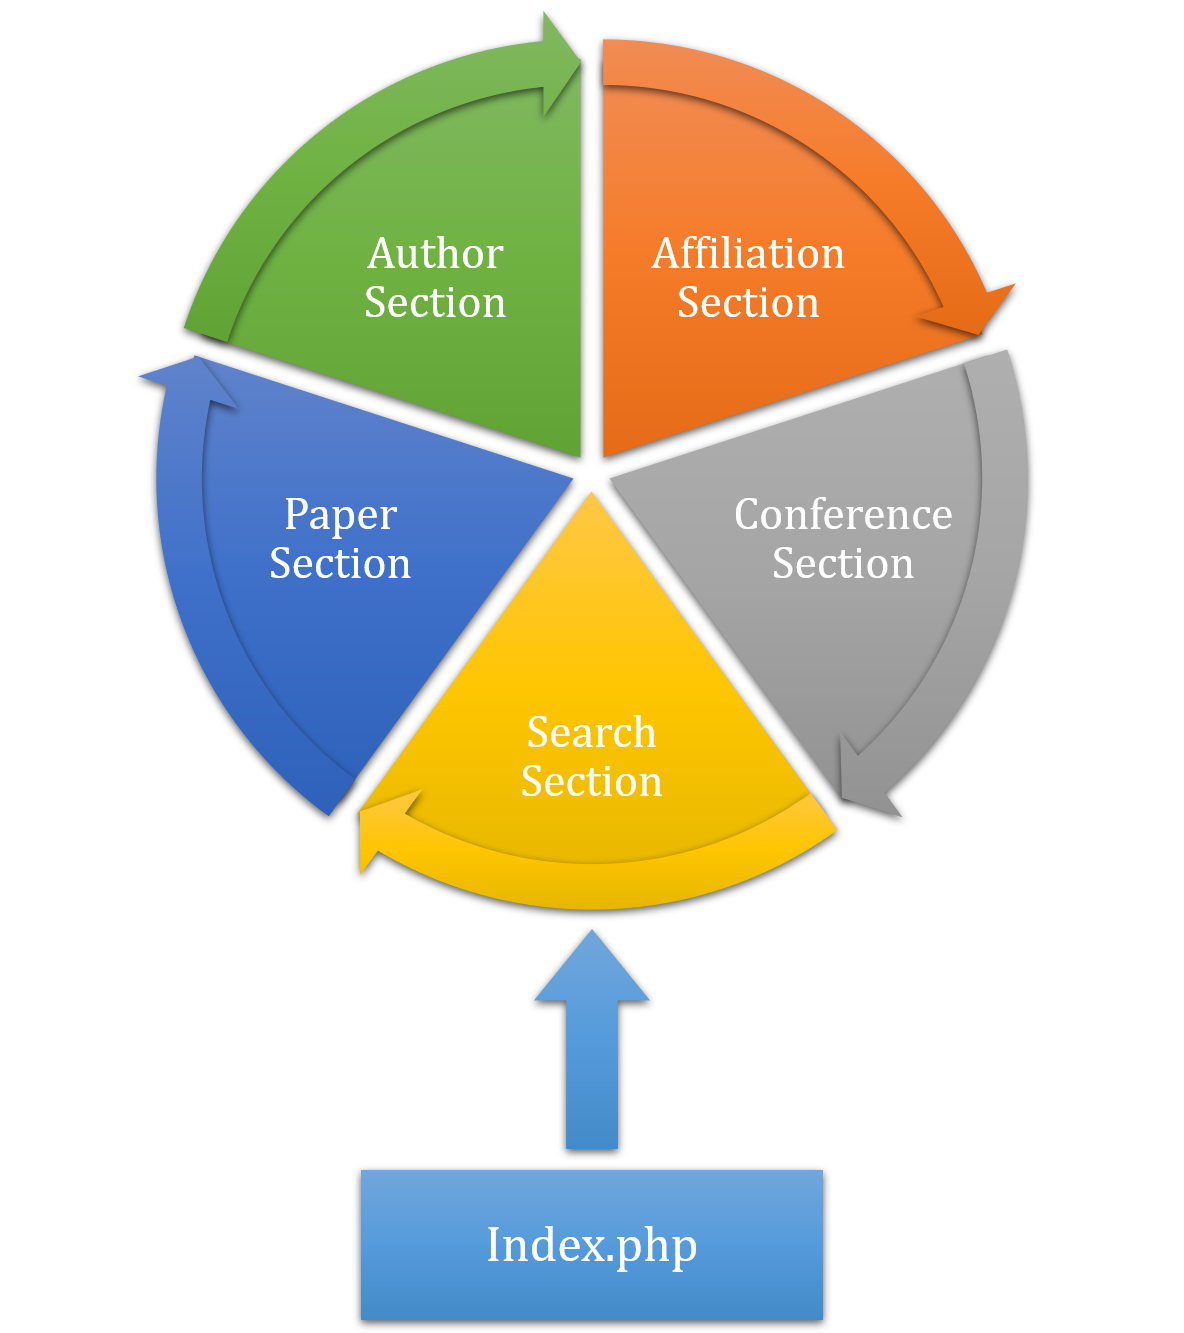
\includegraphics[scale=0.5]{img/zlt_pre_1.png}
\caption{General Structure of our Web}
\end{figure}

\paragraph{index.php}

\begin{itemize}
\item An Integrated Search Bar \textit{by Shaoheng Fang}
\item A 3D-Graph Showing the Distribution of Years and Conferences \textit{by Shaoheng Fang}
\item The Transplantation \& modification of an online Template  \textit{by Shaoheng Fang}
\end{itemize}

\paragraph{Search Section}
\begin{itemize}
\item Search Results Formatting \textit{by Litao Zhou}
\item Visulized Graphs \textit{by Shaoheng Fang}
\begin{itemize}
	\item Publish Year
	\item Conference
	\item Top Authors
\end{itemize}
\item Leaf Flipping in Search Results \textit{by Shiwen Dong}
\end{itemize}

\paragraph{Paper Section}
\begin{itemize}
\item Paper Information \textit{by Litao Zhou}
\item Paper Relation Chart \textit{by Litao Zhou}
\item Leaf Flipping in multiple Pages \textit{by Shiwen Dong}
\item Paper Reference/Citations/Recommendation  \textit{by Hongbo Yang}
\end{itemize}

\paragraph{Author Section}
\begin{itemize}
\item Author Information \textit{by Litao Zhou}
\item Visulized Graphs \textit{by Shaoheng Fang}
\begin{itemize}
	\item Publish Year (Pie Chart \& Bar Chart)
	\item Conference (Pie Chart \& Bar Chart)
\end{itemize}
\item Leaf Flipping in Author Publications \textit{by Shiwen Dong}
\end{itemize}

\paragraph{Affiliation Section}
\begin{itemize}
\item Affiliation Author List \& Conference List \textit{by Litao Zhou}
\item Visulized Graphs \textit{by Shaoheng Fang}
\begin{itemize}
	\item Publish Year
	\item Top Author by Reference
	\item Top Author by Publication
\end{itemize}
\item Leaf Flipping in Author List and Conference List \textit{by Shiwen Dong}
\end{itemize}

\paragraph{Conference Section}
\begin{itemize}
\item Paper Table \textit{by Litao Zhou}
\item Paper Publish Year Graph \textit{by Shaoheng Fang}
\item Author Relation Big Graph by Gephi \textit{by Hongbo Yang}
\item Leaf Flipping in Paper Table \textit{by Shiwen Dong}
\end{itemize}


\section* {How we work together}

The making of a website requires frequent communication of source codes. In response, we use Github as a platform to exchange our codes. At the beginning of our project, we took some time to learn how Git works and created a uniform database and solr engine to make our codes work on everyone's computer. Then every member will be working and making progress on his own branch. We can use the Git system to merge our progress onto the master branch when necessary, and distribute the new version to everyone's branch. With the help of the Git system, we no longer have to bother comparing different codes written by multiple collaborators or having trouble with the inconsistency in others' codes. The network graph was derived from our Github repository homepage, where our commits and branches are displayed.

\begin{figure}[H]
\centering
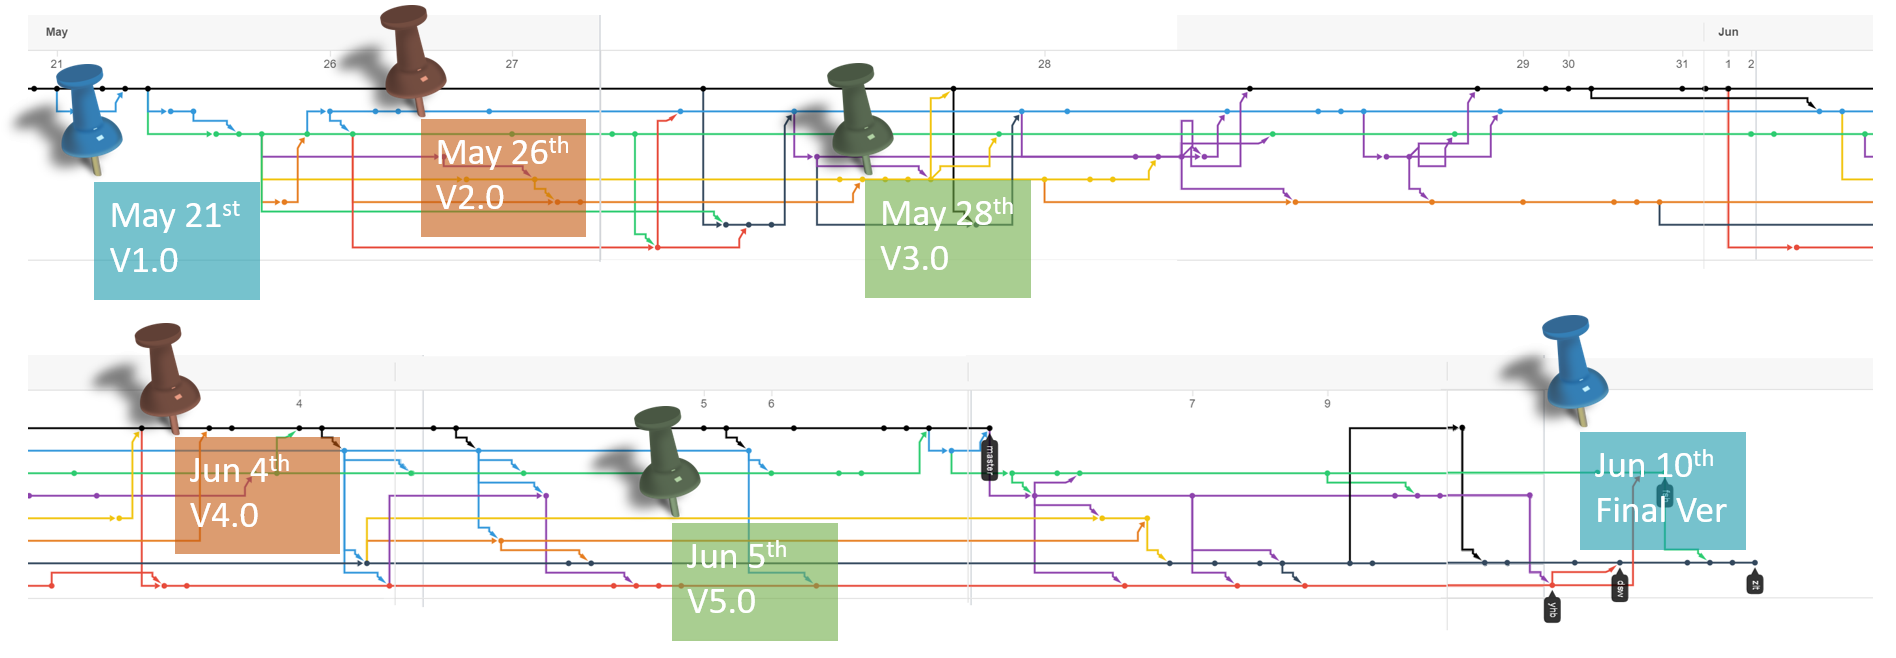
\includegraphics[scale=0.25]{img/zlt_pre_2.png}
\caption{Our Developing Story}
\end{figure}

\section* {How to Check our Work}

To see our source codes, you can visit our github repository homepage (https://github.com/ltzone/EE101Lab) and clone our repository down to your computer. You may also find the LaTeX source codes of this report in our repository. In order to make our website work on your computer, you have to follow our guide in the configguide.txt. This guide will help you initialize your MySQL database and Solr engine and write all the information into them. You may also check our presentation slides to see the detail of our developing story.


\mainmatter
\chapter {Enrich the Contents}

\section {Paper \& Conference Pages}

These parts are required as a necessary part of final lab. We want to display useful information to users. So we added functions to search for more detailed relavant messages. According to the characteristics of each field, we used different methods to show information.


\subsection{Description}
In our final version, there are 5 concrete pages about paper information and 3 about conferences. We tried to display the information in all directions. There are blanks to show basic information, E-charts of papers, citations and references and relavant recommedations. 

\subsection{Paper: Basic Information}
In this page, we show basic messages of papers
which is from MySQL table `papers' and ` paper\_author\_affiliation'.
 And we offer the function to jump to Conference, Author, Affiliation Pages and Acemap.


The codes are listed below. (Realization of Paper Charts will be introduced in chapter visualization.)

First, we have PaperID through ``Get'' method, then we can find result in MySQl. If result exists, we echo out all fields of paper-relavant  information. (Remember that  AuthorName is in the format of Arrays.)

\begin{figure}[H]
\centering
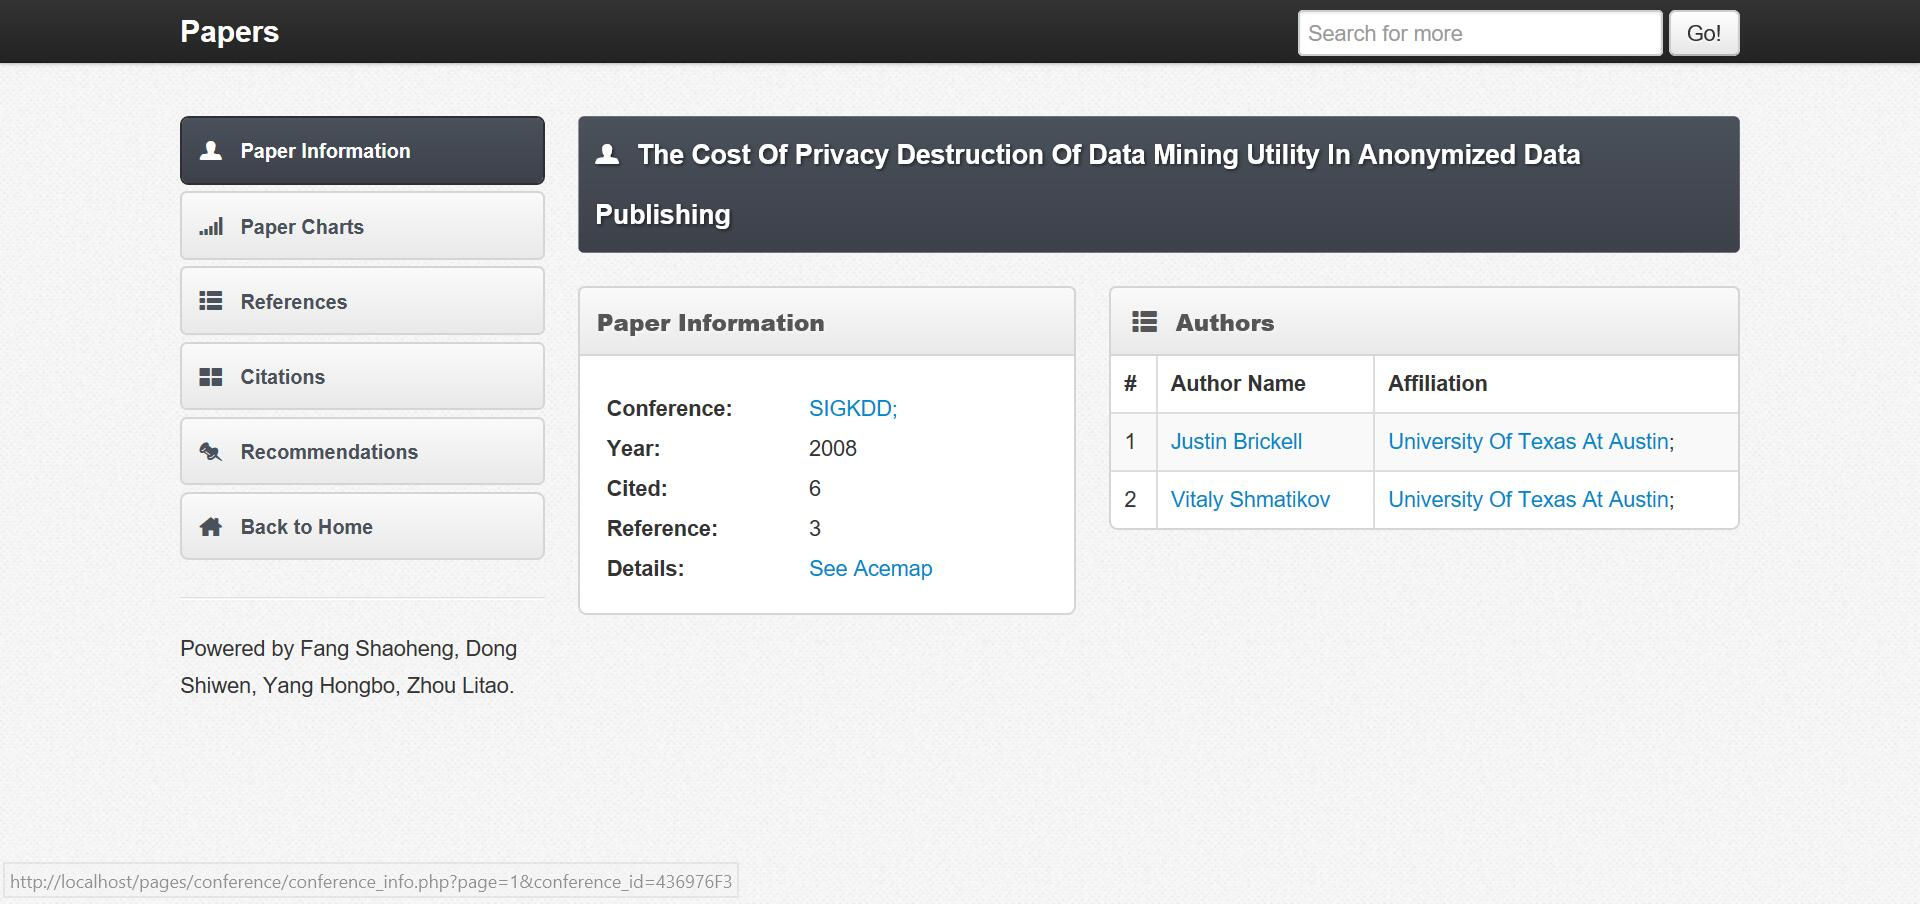
\includegraphics[width=11.0cm]{img/yhb_paper_1.jpg}
\caption{Page Example}
\end{figure}


\begin{figure}[H]
\centering
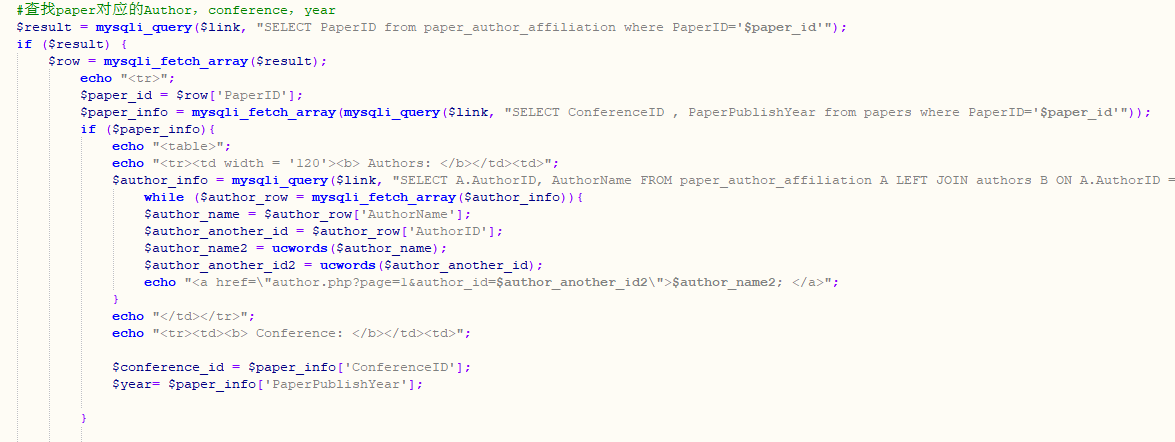
\includegraphics[width=11.0cm]{img/yhb_mp_1.png}
\caption{Code Example}
\end{figure}

\begin{figure}[H]
\centering
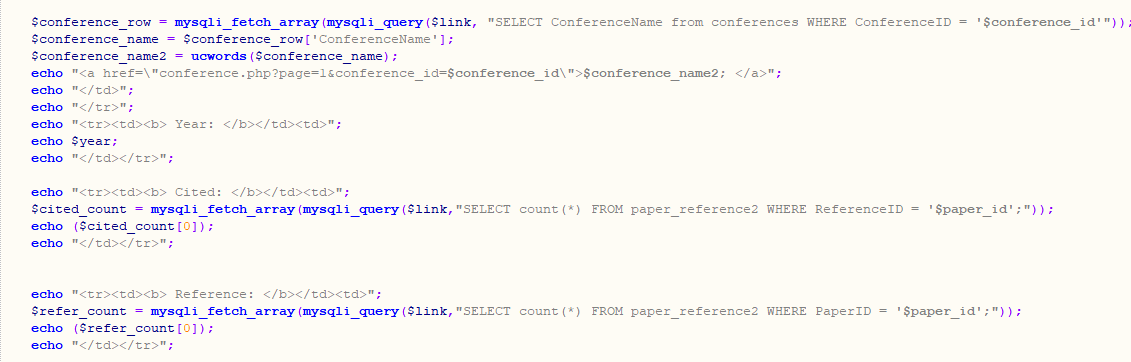
\includegraphics[width=11.0cm]{img/yhb_mp_2.png}
\caption{Code Example}
\end{figure}



\subsection{Paper: Citation and Reference}
This part is quite similar to paper information part(just add a while loop).
Before doing this, we should know what is thrown into MySQL. In the fuction above, that is PaperID, and in Reference part, it's ReferenceID while in Citation part, we swap paper and reference.

\begin{figure}[H]
\centering
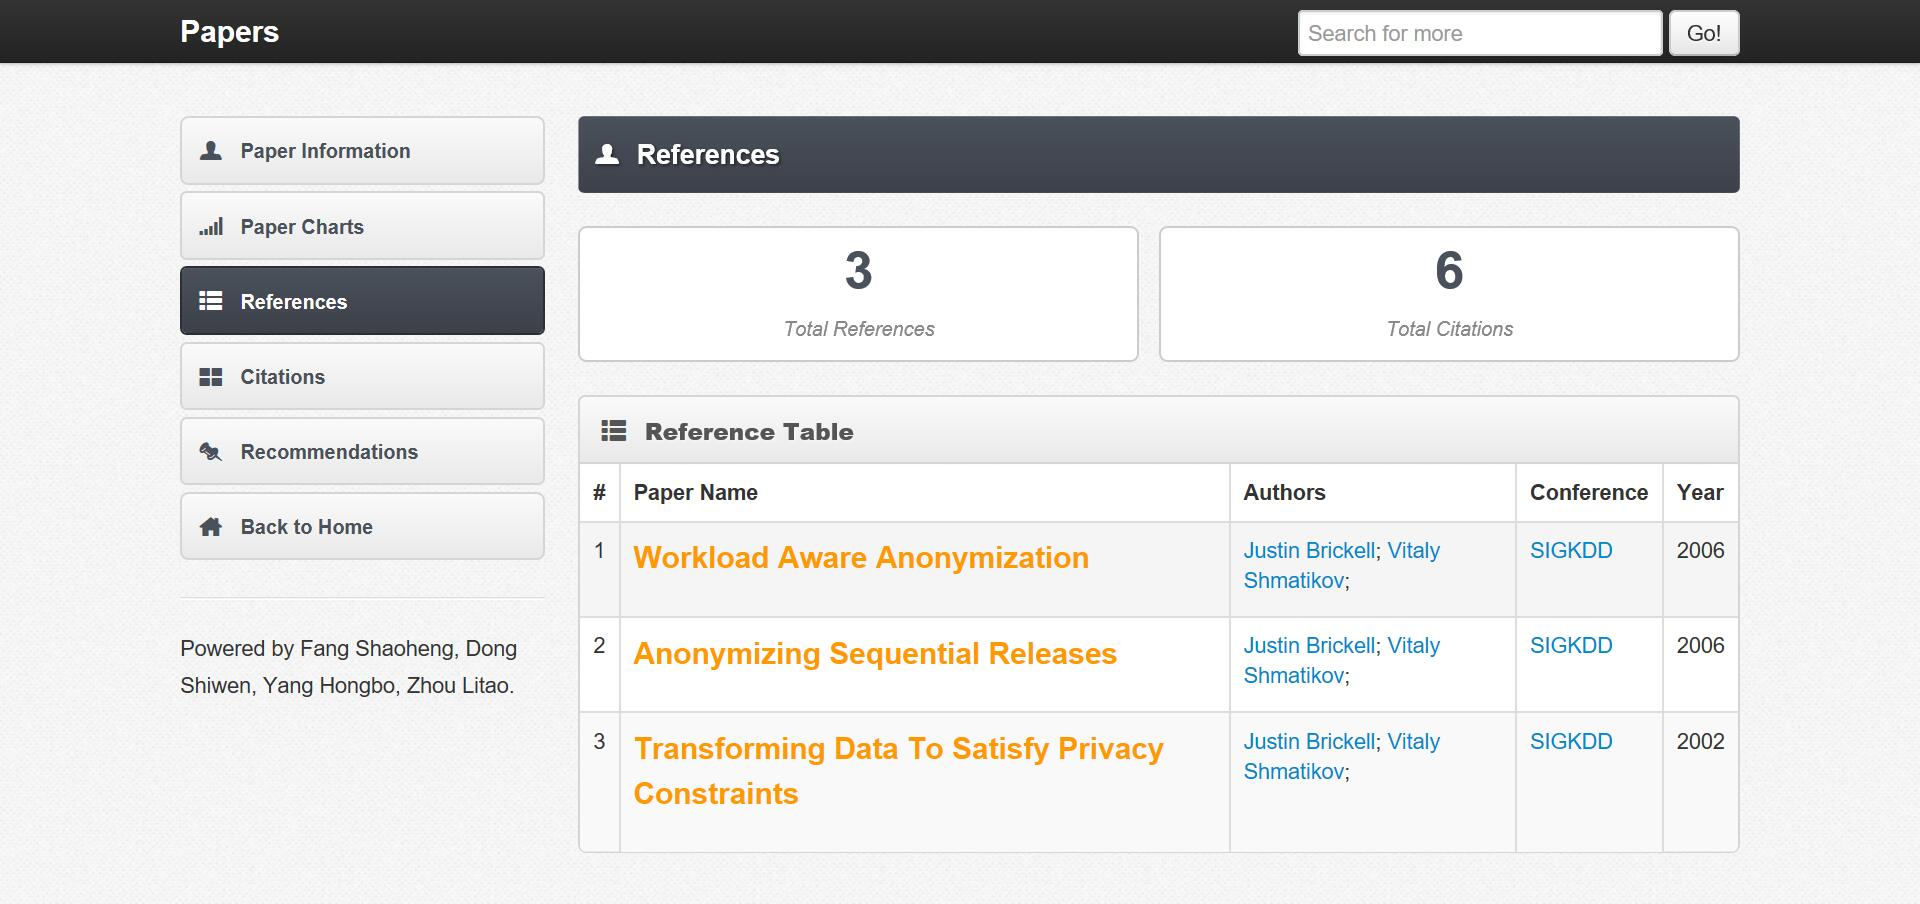
\includegraphics[width=11.0cm]{img/yhb_paper_2.jpg}
\caption{Page Example}
\end{figure}
Here we give code: (just the first part, the followed part has been already introduced.)
\begin{figure}[H]
\centering
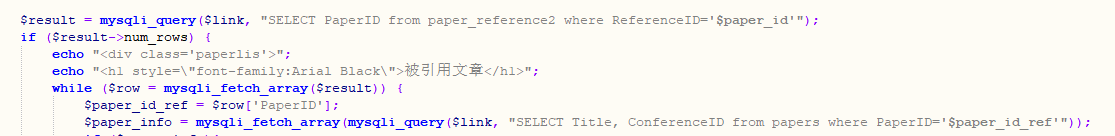
\includegraphics[width=11.0cm]{img/yhb_re_2.png}
\caption{Code Example}
\end{figure}

This is Citation Page example:
\begin{figure}[H]
\centering
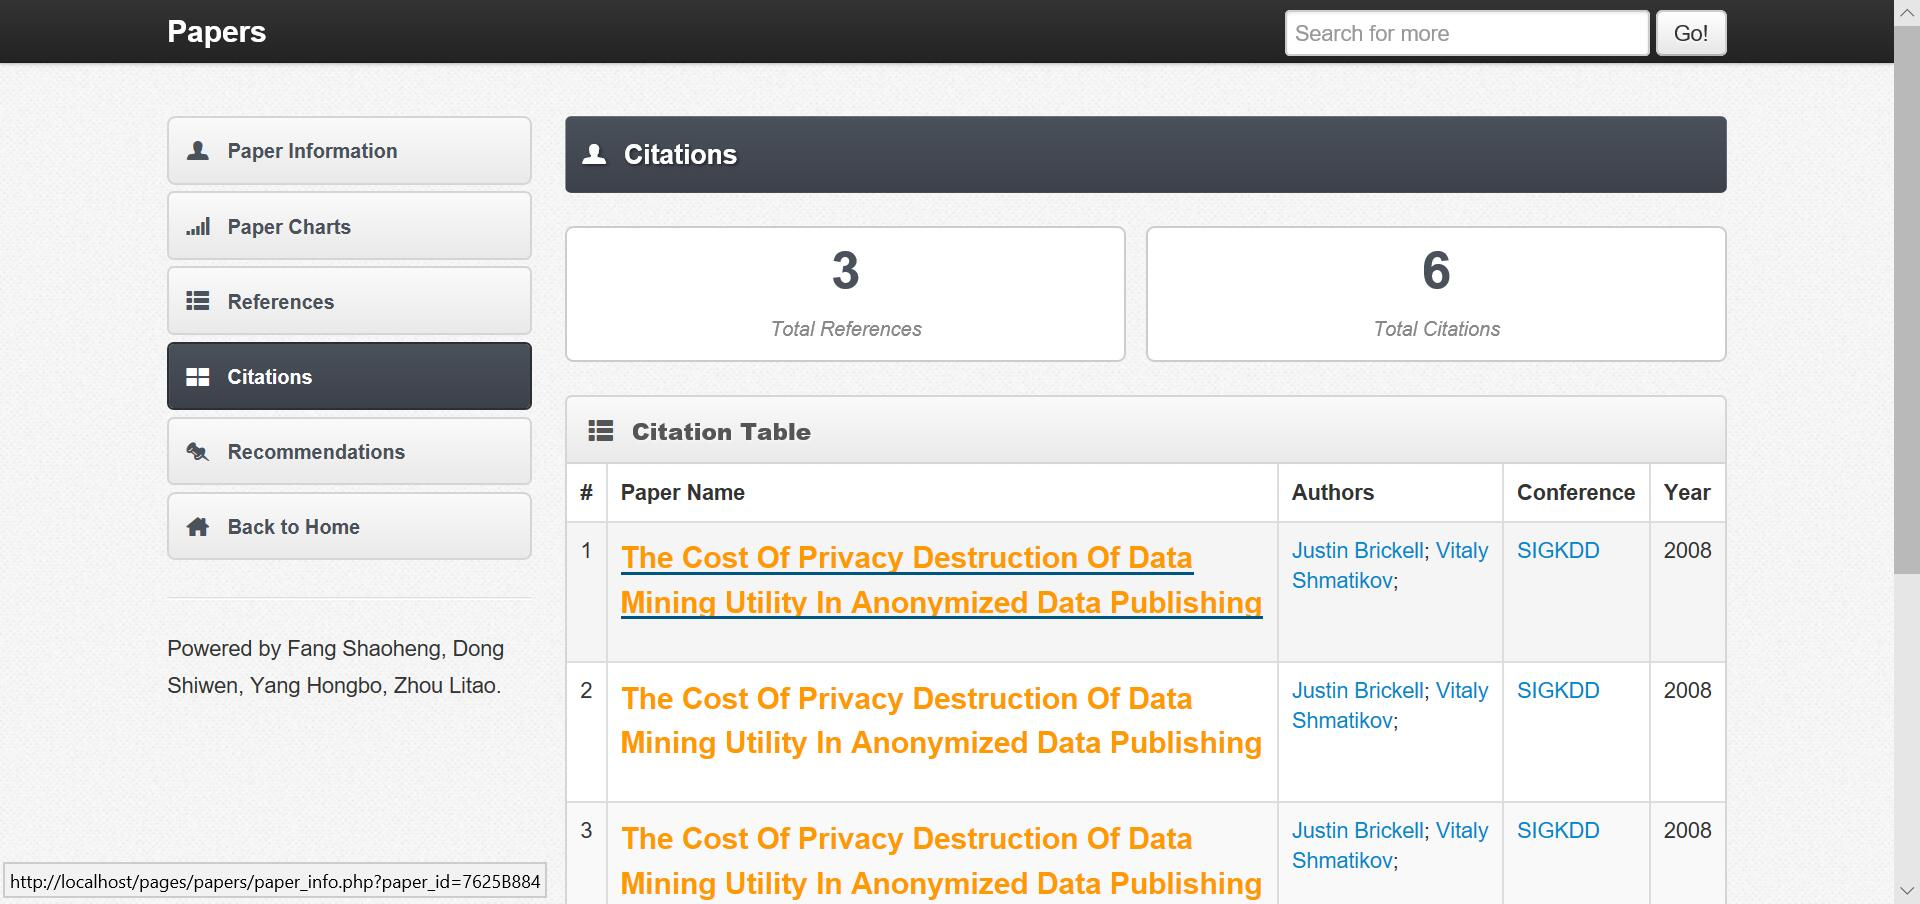
\includegraphics[width=11.0cm]{img/yhb_paper_3.jpg}
\caption{Page Example}
\end{figure}
Here we give code:
\begin{figure}[htp]
\centering
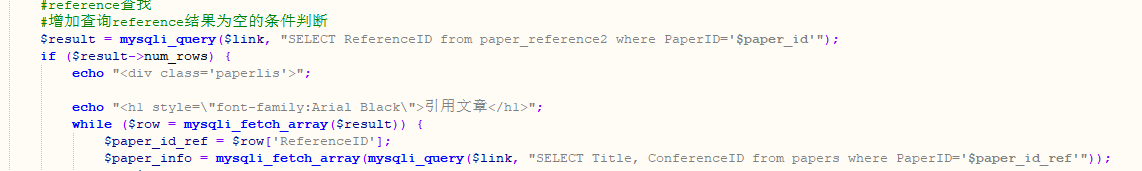
\includegraphics[width=11.0cm]{img/yhb_re_1.png}
\caption{Code Example}
\end{figure}


\subsection{Paper: Recommendation}
We came up with 2 method to recommend papers: 

\textbf{1) Recommend by relavant title}

This method relies on solr. In solr, field Title is stored as `text-en' format. So we can do vigrous search to match related papers First, we should search in MySQL to find Title (at the beginning, we have paper\_id ).
As the search result is in the format of (``    xxxxx   ''), 
we should process it to xxxxx to transmit to solr-url.
Specificly, we use   (var:)paper\_title4=substr((var:)paper\_title3,3,-2);


\begin{figure}[htp]
\centering
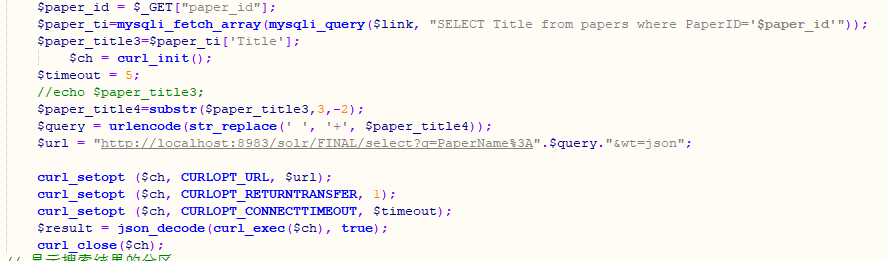
\includegraphics[width=11.0cm]{img/yhb_re_11.png}
\caption{Code Example}
\end{figure}

Then similarly, we can echo result out. (See Figure \ref{fig:yhb1} on the next Page)

\begin{figure}[h]
\centering
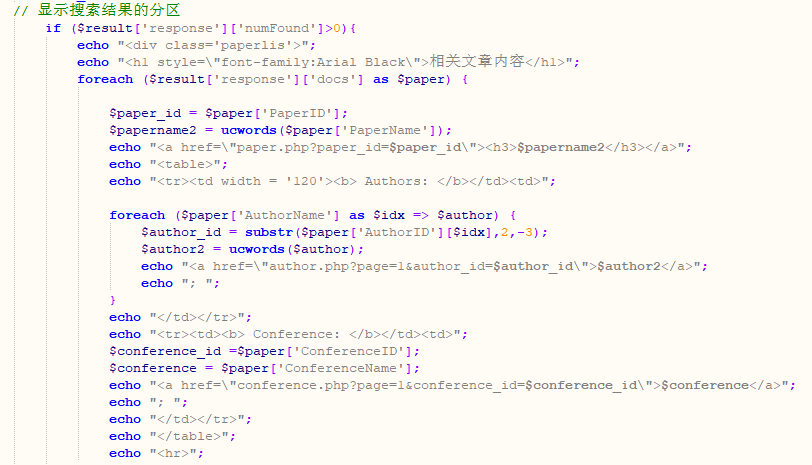
\includegraphics[width=11.0cm]{img/yhb_re_12.png}
\label{fig:yhb1}
\caption{Code Example}
\end{figure}


\textbf{2) Recommend by relavant Author}

This method relies on MySQL. The central sentence of this part is the MySQL join-query sentence below:
\begin{figure}[H]
\centering
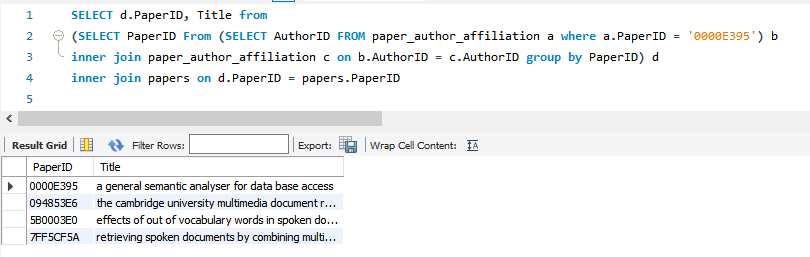
\includegraphics[width=11.0cm]{img/yhb_mp_4.png}
\caption{Code Example}
\end{figure}



Here we give complete codes:
\begin{figure}[H]
\centering
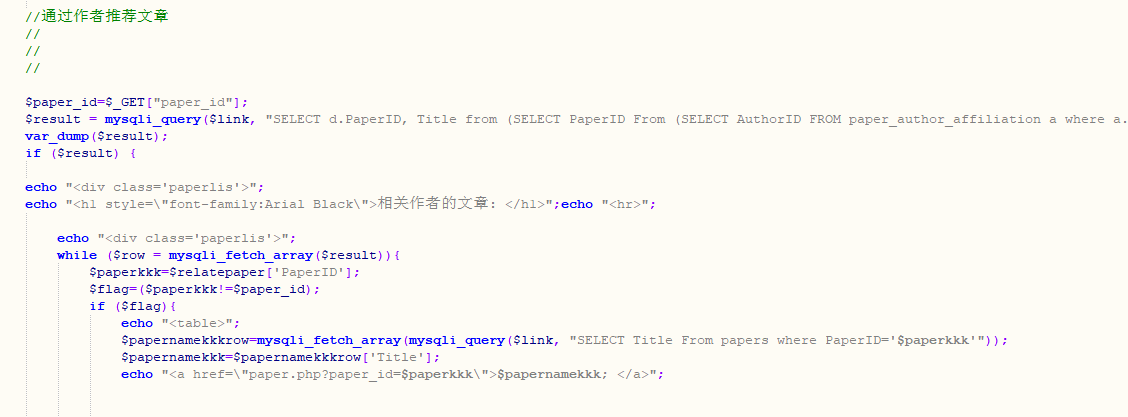
\includegraphics[width=11.0cm]{img/yhb_mp_3.png}
\caption{Code Example}
\end{figure}


Here we give exammple page:
\begin{figure}[H]
\centering
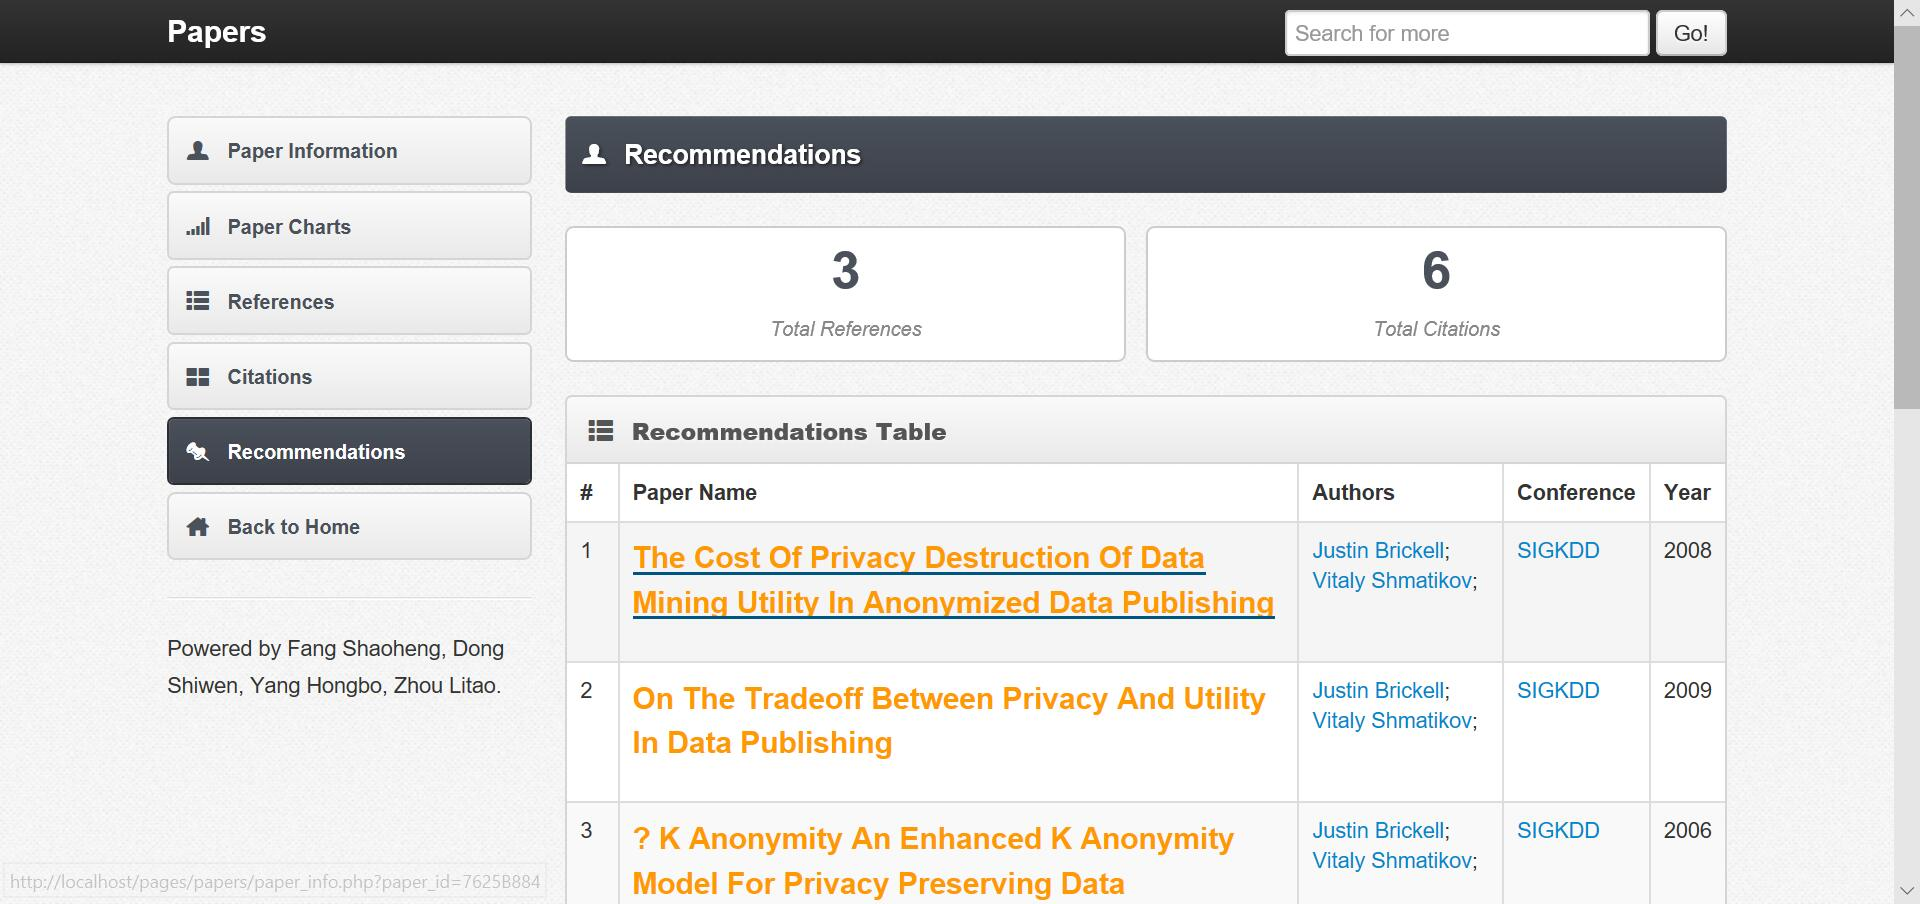
\includegraphics[width=11.0cm]{img/yhb_paper_4.jpg}
\caption{Page Example}
\end{figure}



\subsection{Conference Information}

In conference page, we showed basic information of conferences nameiy the number of authors, papers and references. Then we listed the papers that are included in the distinct conference and gave hyperlinks to other pages.

(The impletment of count function is shown in the next subsection.)
\begin{figure}[H]
\centering
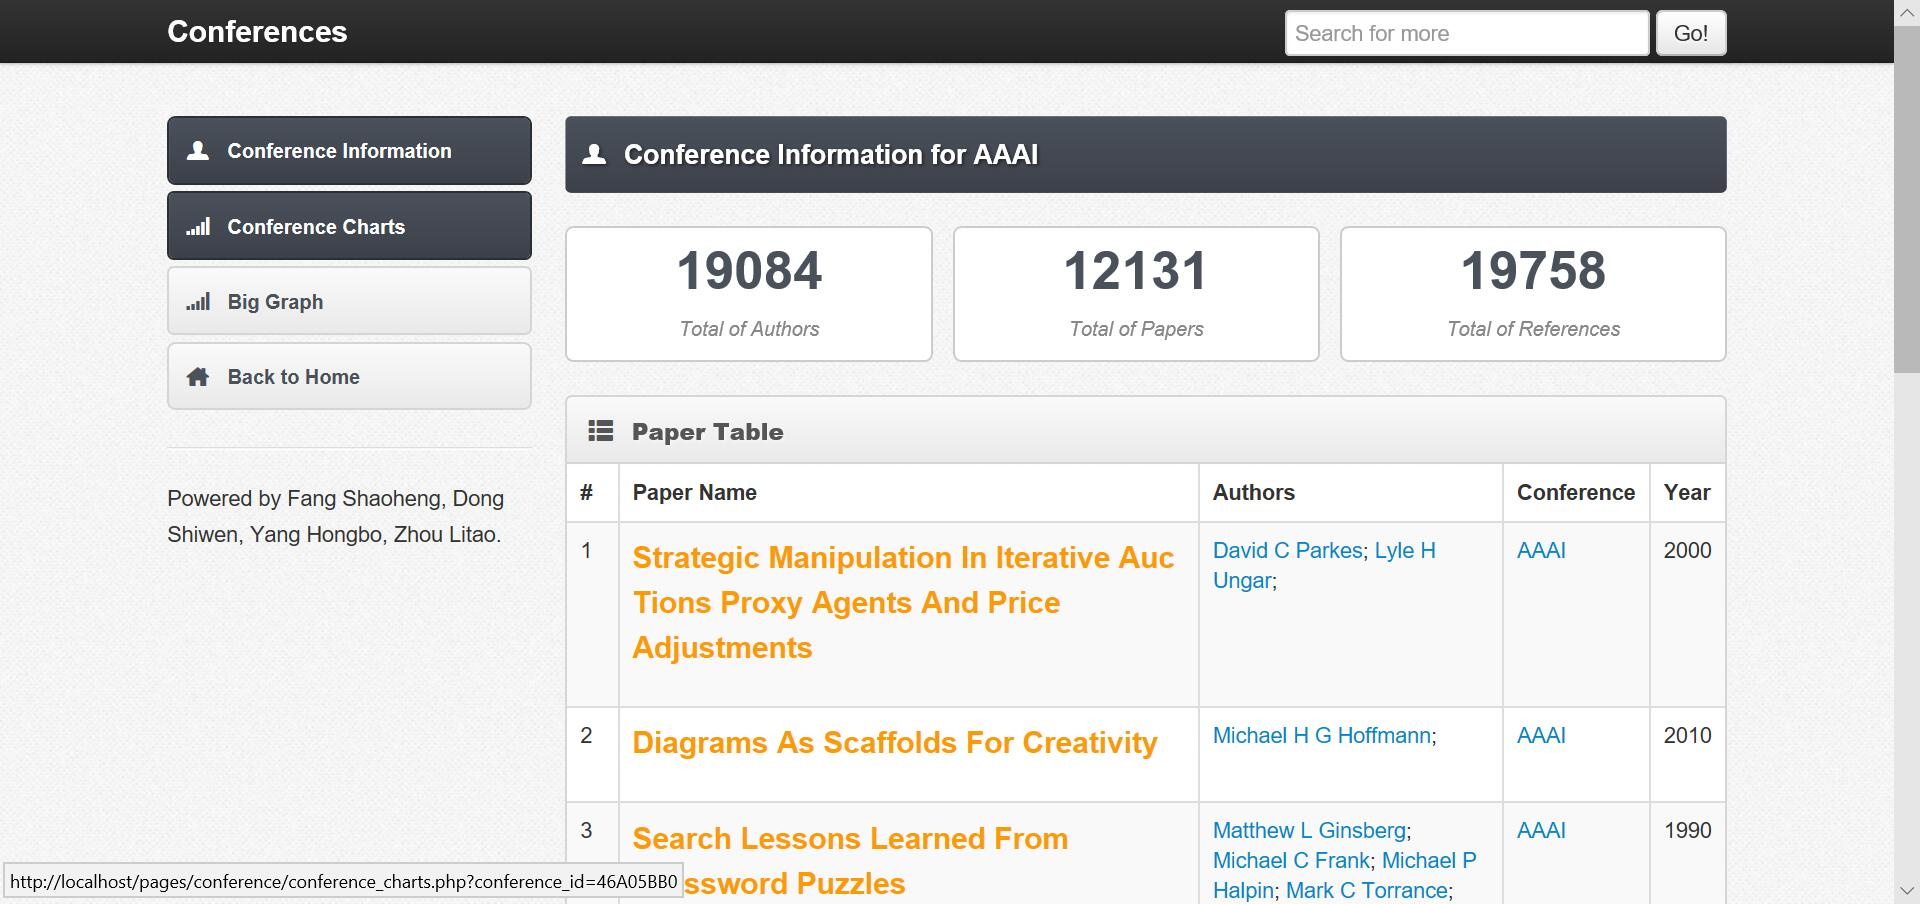
\includegraphics[width=11.0cm]{img/yhb_con_2.jpg}
\caption{Page Example}
\end{figure}
There are 3 blanks on the right side, which show the total number of authors, papers and references. We call this ``count function''. We wrote 2 versions. The first version use counting varaible in loops to count number, which is not  so efficient. So we turned to another method, which will be introduced in detail in ``affiliation page''.

Below these is a paper list.
Here is the code to search for papers that are included in the conference, the process to achieve  it is similar to that of ``author.php'' in last homework. We used MySQL to find the information we want. 

First, we have ConferenceID through `Get', then we can use code:
\begin{figure}[H]
\centering
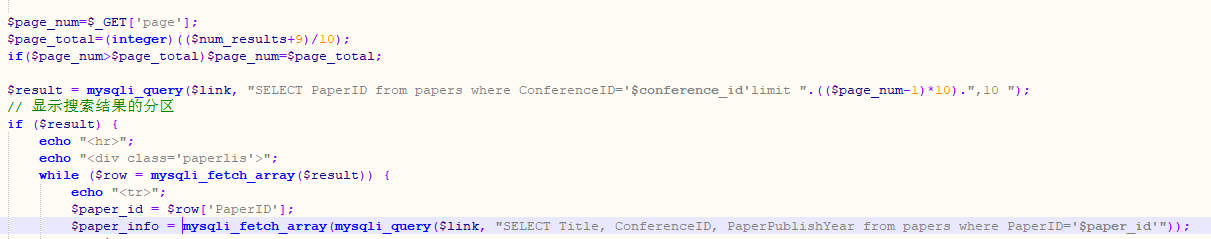
\includegraphics[width=11.0cm]{img/yhb_con_11.png}
\caption{Code Example}
\end{figure}


to find PaperID. And problem comes to using PaperID to find paper information.  We just follow the approach that was used in last homework, and echo the needed messages out. There is a point that should be mentioned. AuthorID field has multiple value, so we have to process like an array.
\begin{figure}[H]
\centering
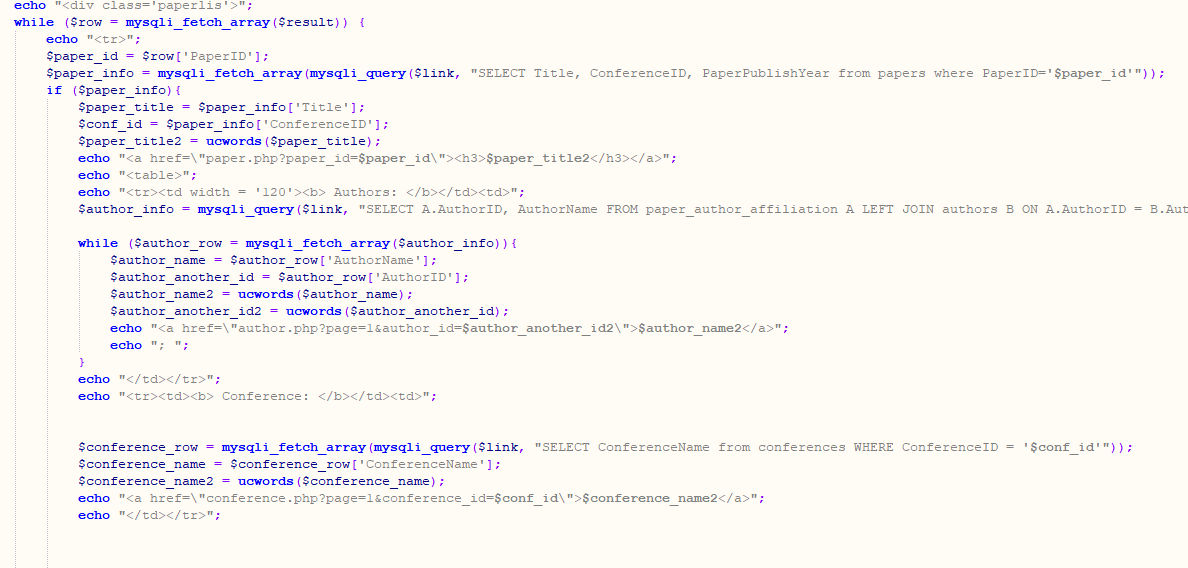
\includegraphics[width=11.0cm]{img/yhb_con_1.png}
\caption{Code Example}
\end{figure}


We also added E-charts and Gephi graphs in related pages to show the information of conference more clearly, which method will be discribed in detail in following chapters.

\section {Affiliation Pages}

We'd like to add a new series of pages to show affiliation information to users. Since we didn't do any previous work about affiliation information in the previous labs except that the affiliation table was input into the database, we have to write new SQL commands in search of affiliation information, and echo them out on the pages. The paper table and charts on other pages can be of help in showing the affiliation related information. Also, we have already got the author table written in the paper information page. Generally speaking, the work here is to collect the affiliation data and arrange them in order on the pages.


\subsection {General Description}

The final version of the affiliation section include 3 concrete pages. On the affiliation\_info.php page, we will give three numbers on top of the page, counting all the authors, papers, and references in the affiliation. Then the authors in the affiliation will be listed below, together with their own affiliation information (hyper-links included) and number of publications. Affiliation\_paper.php shows all the papers related to the affiliation. The affiliation\_charts.php, where three charts are displayed, will be reported in detail in the Statistical Graph Section.
(See Figure \ref{fig:zlt1} and Figure \ref{fig:zlt2} on the next Page)



\begin{figure}[h]
\centering
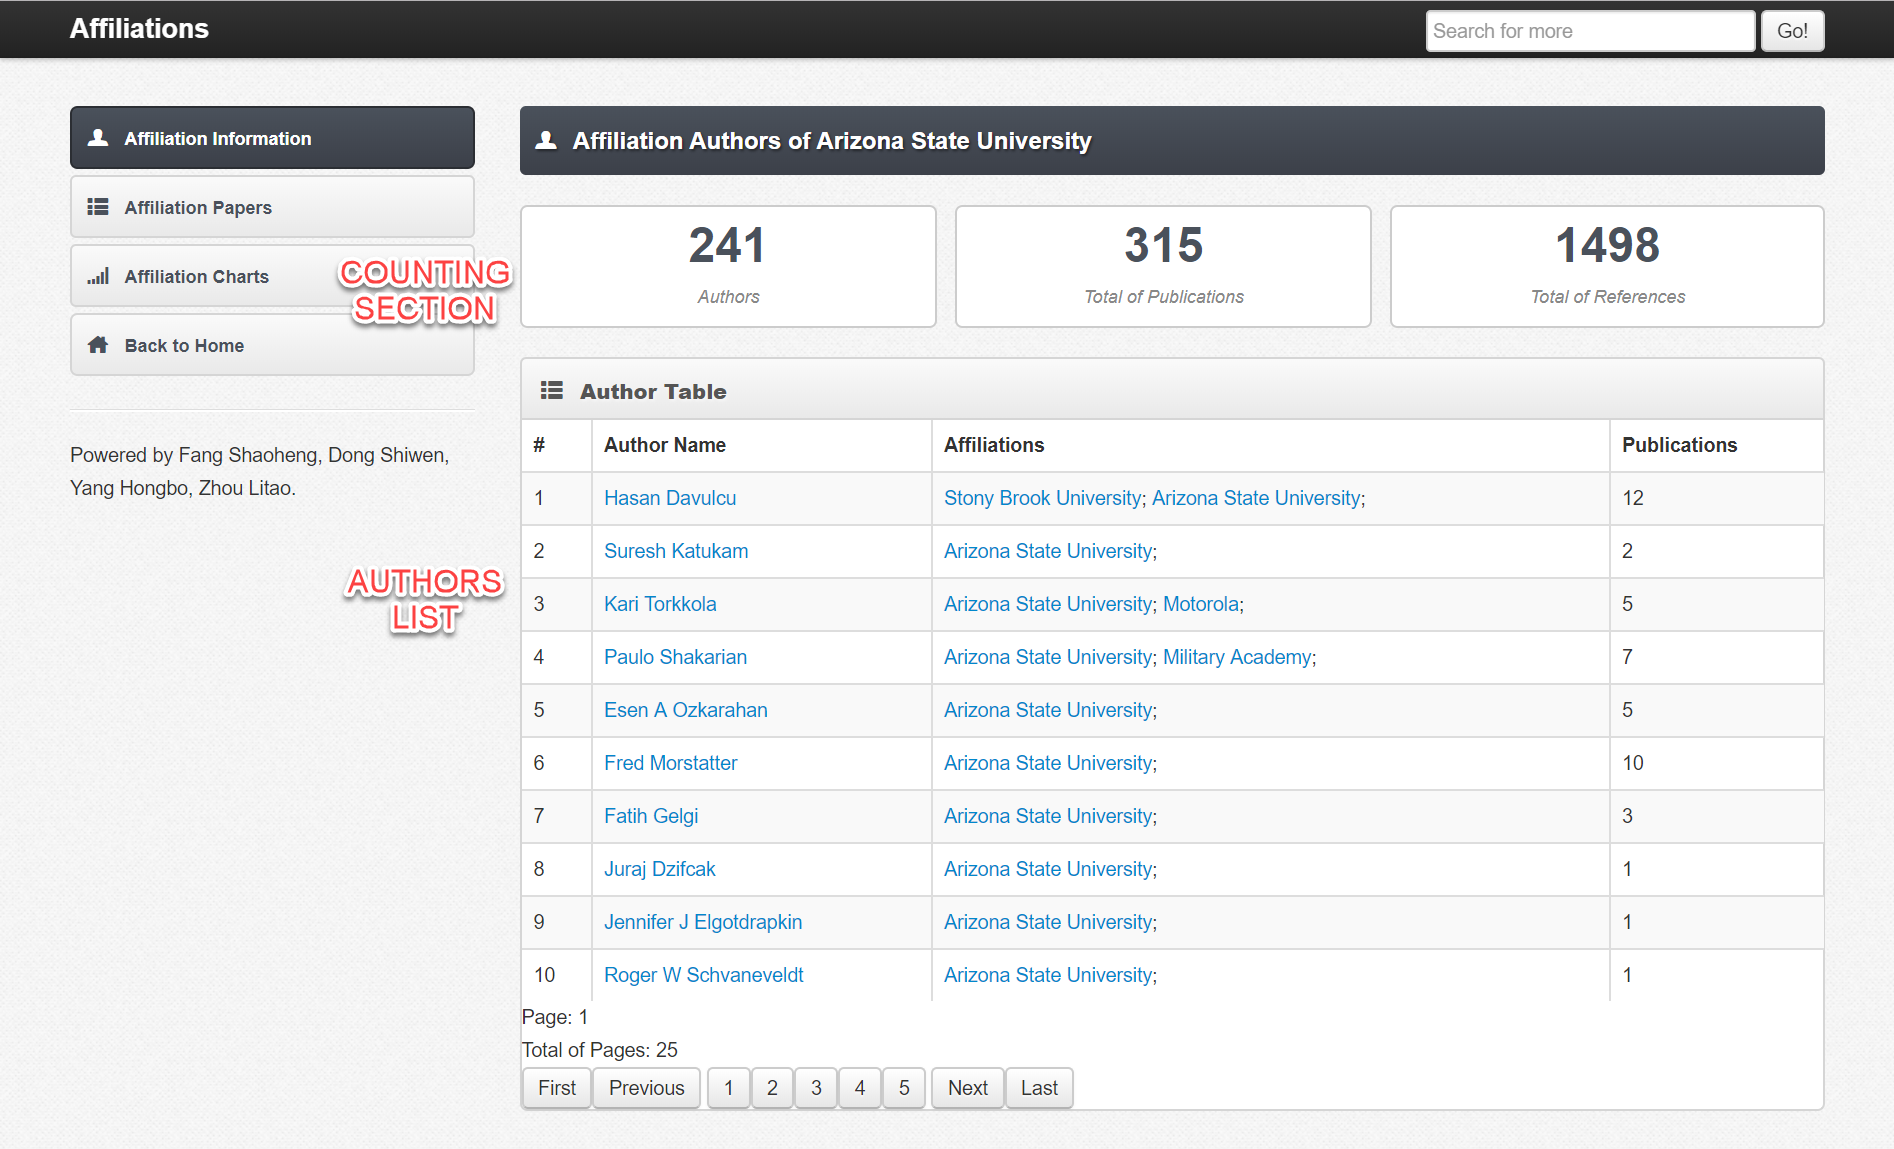
\includegraphics[scale=0.35]{img/zlt_aff_demo1.png}
\caption{affiliation\_info.php page}
\label{fig:zlt1}
\end{figure}

\begin{figure}[h]
\centering
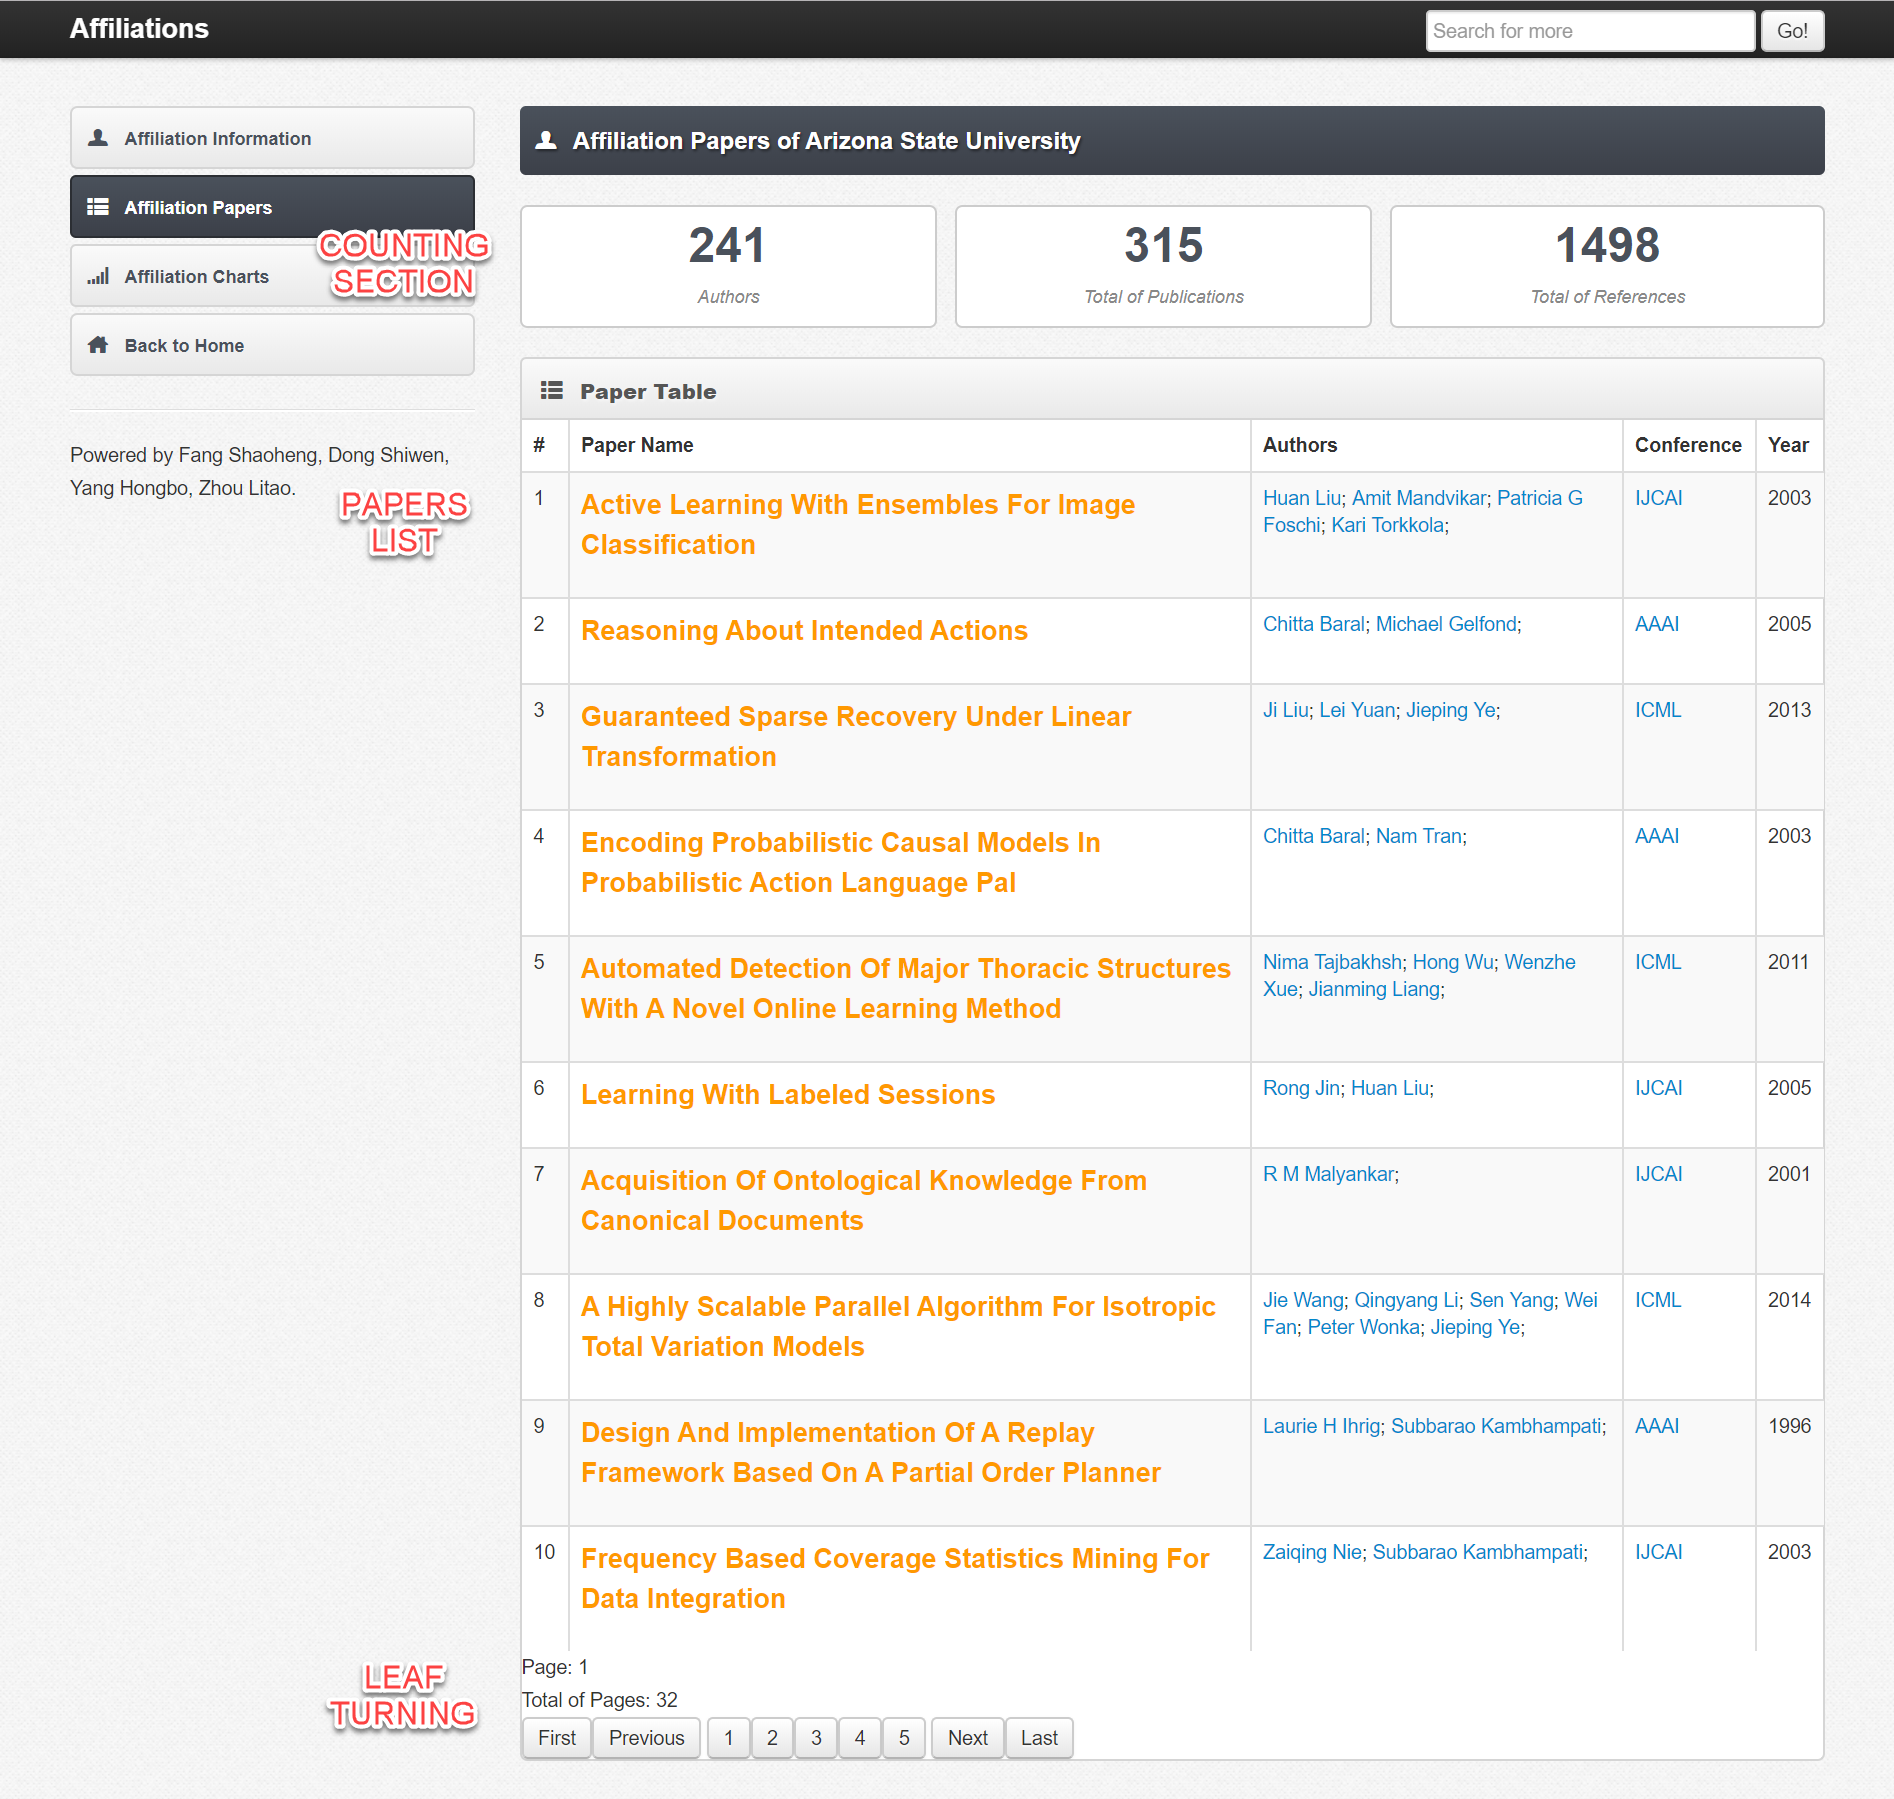
\includegraphics[scale=0.35]{img/zlt_aff_demo2.png}
\caption{affiliation\_paper.php page}
\label{fig:zlt2}
\end{figure}

In fact, for the same function to be displayed on the page, we did two versions of code to implement them. The first one was very basic, just like those in the paper/author/search pages. However, since all the affiliation data are selected from the big paper\_author\_affiliation table, the first version didn't perform well in loading speed. Our optimization will be introduced in the Optimization Chapter.



\subsection {Total Counts}
On top of every affiliation page, we've counted all the authors, papers and references concerned. For authors and papers, we can directly count them in the paper\_author\_affiliation table. For references, we first select the papers and then join the selected results to the paper\_reference table in order to count the results. The MySQL commands are listed below.

\begin{figure}[H]
\centering
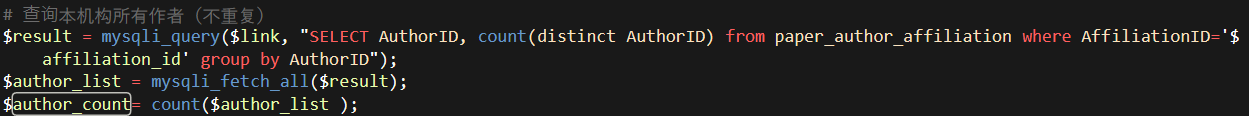
\includegraphics[scale=0.55]{img/zlt_aff_authorcount.png}
\caption{Count Author Commands}
\label{fig:aff_authorcount}
\end{figure}
\begin{figure}[H]
\centering
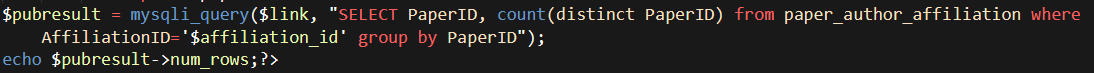
\includegraphics[scale=0.6]{img/zlt_aff_papercount.png}
\caption{Count Paper Commands}
\label{fig:aff_papercount}
\end{figure}
\begin{figure}[H]
\centering
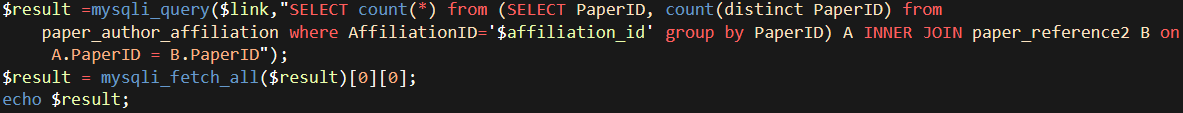
\includegraphics[scale=0.55]{img/zlt_aff_refcount.png}
\caption{Count Reference Commands}
\label{fig:aff_refcount}
\end{figure}

Note that we've use some MySQL techniques such as DISTINCT (eliminate overlapping results) and GROUP BY (perform data counting job) in order to implement our function.

For the data display in our page, our template has already provided a well designed data container in CSS, which can list different numbers in a row, with even width. We can simply apply this pre-defined class in a way demonstrated below.

\begin{figure}[H]
\centering
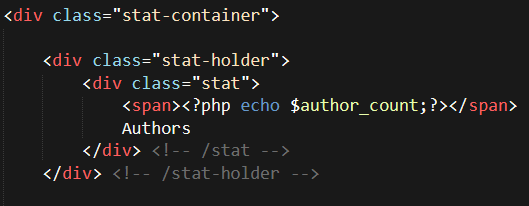
\includegraphics[scale=0.8]{img/zlt_aff_countdisplay.png}
\caption{Use Pre-defined Class to Display Numbers}
\end{figure}


\subsection{Authors List}

The author we've found based on the given affiliaiton may have more than one affiliation where he publishes his paper. So one simple search work is not enough. Luckily, all of the data related to this problem can be selected from the paper\_author\_affiliation table. As a result, our first design is to first sort out all the authors where the affiliation column fits, then we search the table again for affiliation information based on the author's id, which can be realized by looping through the author array in PHP.

In fact, the first step has been done when we count the authors (See Figure \ref{fig:aff_authorcount}), so we simply skip the first step, call the author selecting result in the counting section, and make further searching based on the previous result. During the second step, we've also used DISTINCT \& GROUP BY techniques in order to get the author's affiliation data right and unrepeated.

\begin{figure}[H]
\centering
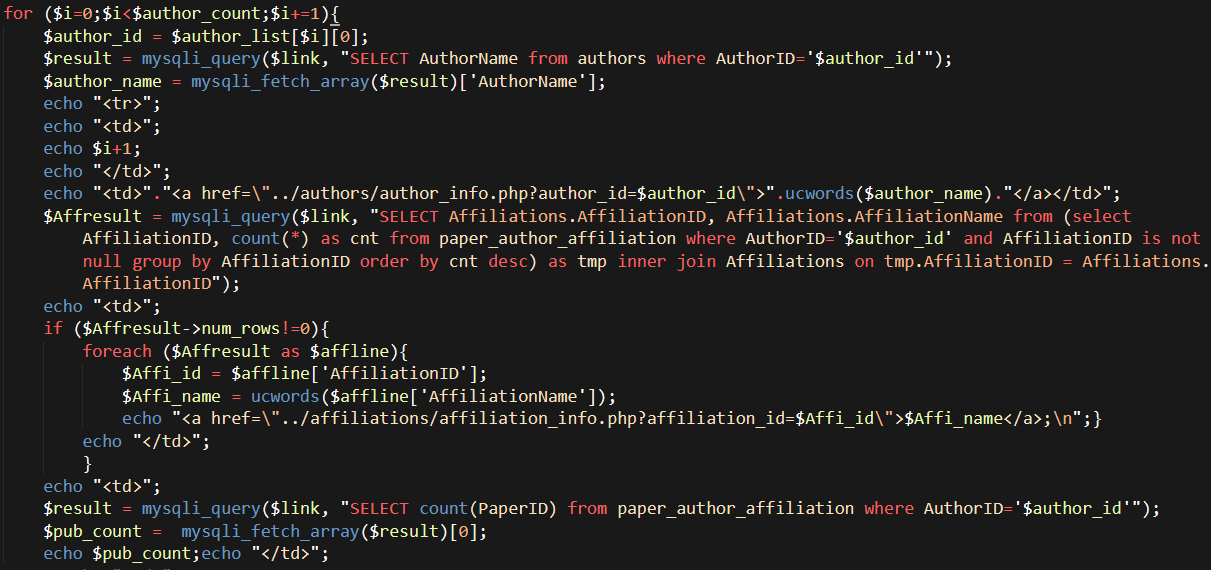
\includegraphics[scale=0.55]{img/zlt_aff_authorloop.png}
\caption{Use Loop to List Author\_Affiliation Information}
\end{figure}

The problem with this solution is that the searching work is too much. Imagine there are 100 authors related to one affiliation, we have to go through the big paper\_author\_affiliation table 100 times in order to get all the data. It turned out that it would take the webpage about half a minute to get completed loaded. The optimization work will be introduced in the Optimization Chapter.

\subsection{Papers List}

The general structure of this list is simlilar to those in citation/ reference/ author's paper list. We may just use MySQL to select all the paper's id related to the affiliation, keep this array storing the paperid we want to display, and the leave the rest of the work to the codes we've already written in the previous work. The selecting MySQL commands are listed below. Actually, just like the case in the author list section, the first step has also been completed in the counting section. (See Figure \ref{fig:aff_papercount}) So there are no codes left for this section to explain.

\chapter{Leaf Turning}

Page turning is an indispensable part of web design. When there is more information to be searched and displayed, the page turning function can reduce the number of information displayed on each page, which makes the whole page look more concise and beautiful, and also optimizes the user's experience.

In this experiment, we have designed two versions of page turning function. And the detailed information of them are as follows.

\section{Version I: by PHP parameters}
In this version,we set the parameter 'page' for each page, and the show scope is determined according to the'page' parameter and each time we don't show all data. Actually, because of specific value of page, we only show 10 pieces of data.
\subsection{Description}
Now let's show the first version's page turning . We take the search results on the'search'page as an example, and the effect is shown in the following figure.
(See Figure \ref{fig:dsw1})

\begin{figure}[h]
\centering
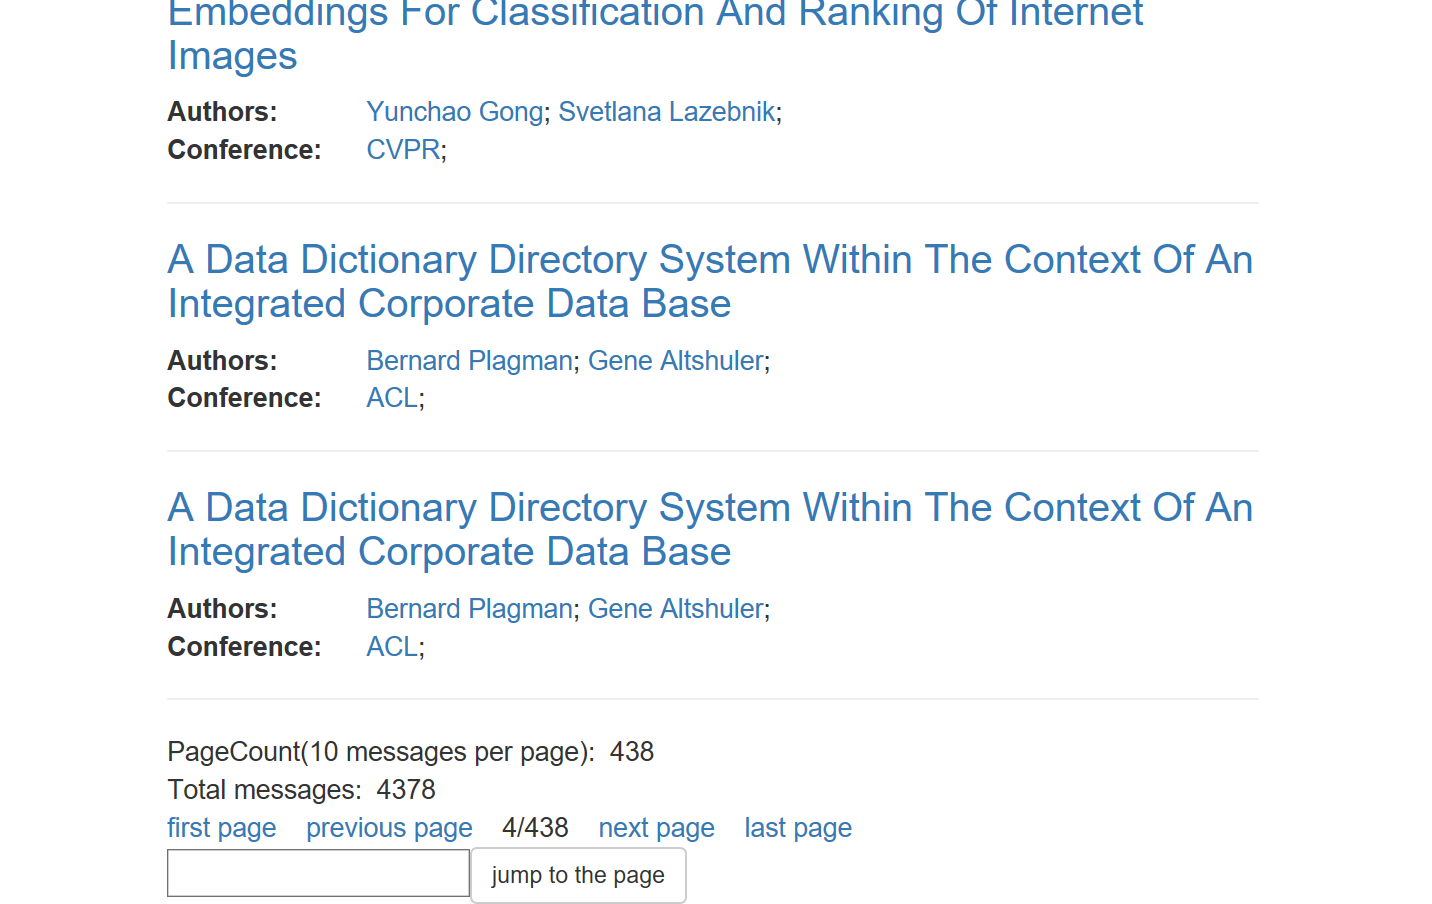
\includegraphics[height=6.0cm,width=10.0cm]{img/dsw_11.png}
\label{fig:dsw1}
\caption{Base Version Demonstration}

\end{figure}
Ten pieces of information are displayed on each page. At the bottom of each page, the number of the current page, total data and total pages can be displayed. By clicking the'previous page's and 'next page's hyperlinks, the page can be turned up and down. By clicking the'first page's and 'last page's hyperlinks, the page can be turned to the first and last pages. In addition, we can also input the page number of the page we want to see in the blank and click the button 'jump to the page' to achieve the page jumping.

In this way, we can search the data spending little time . But the disadvantage of this method is that every time we turn the page, we indeed open a new page, and everying needs to be queried and shown again, even though which maybe needn't the page turning function.

\subsection{Solution}

We set the parameter 'page' for each page, and the show scope is determined according to the'page' parameter to make sure that we get specific 10 pieces of data in order to achieve the page turning. Every page's query statments are different because they contain the 'page' paremeter. And the default value of the 'page' is 1.

The page turning is achieved by hyperlinks, and each time we click the specific word or input the page jumping number, we will turn to a new page with different papremeter 'page'.

\subsection{Source Codes}
Now we still take the search page as an example to present the page turning.  The codes are as follows.

\begin{figure}[ht]
\centering
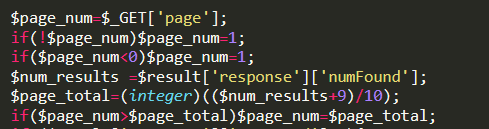
\includegraphics[scale=0.5]{img/dsw_get.png}
\caption{Page Parameter}
\end{figure}

\begin{figure}[ht]
\centering
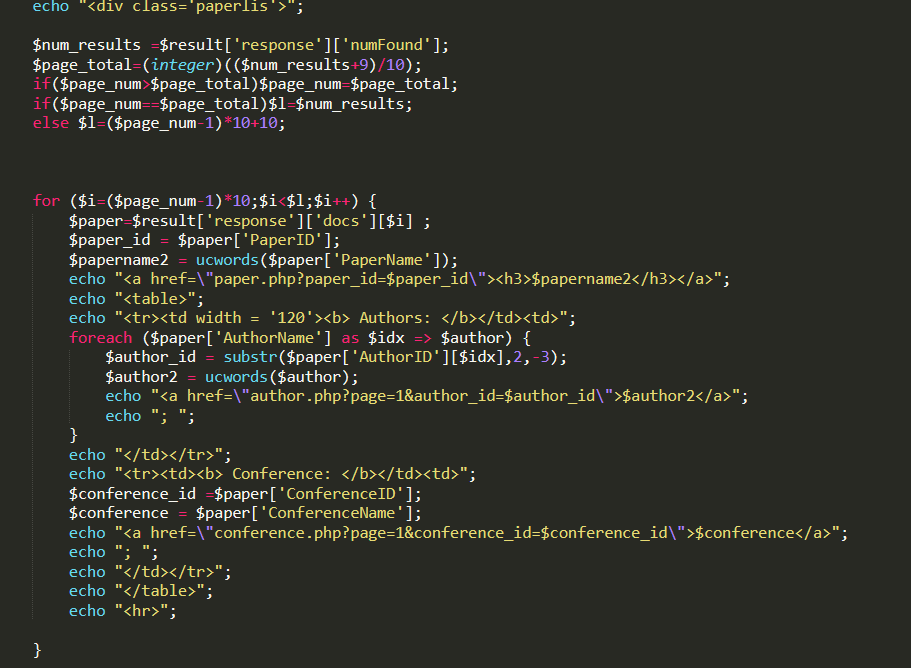
\includegraphics[scale=0.35]{img/dsw_show.png}
\caption{Show}
\end{figure}


At first, we get the paremeter 'page' sent from other pages. Before we search information , we should know the number of total information we get and figure out the number of total pages which depends on how many pieces of data we want to show in a page. Then we use 'for' circle statement to show the data . The codes are shown in the figure'page parameter'and the figure 'show'.



\begin{figure}[ht]
\centering
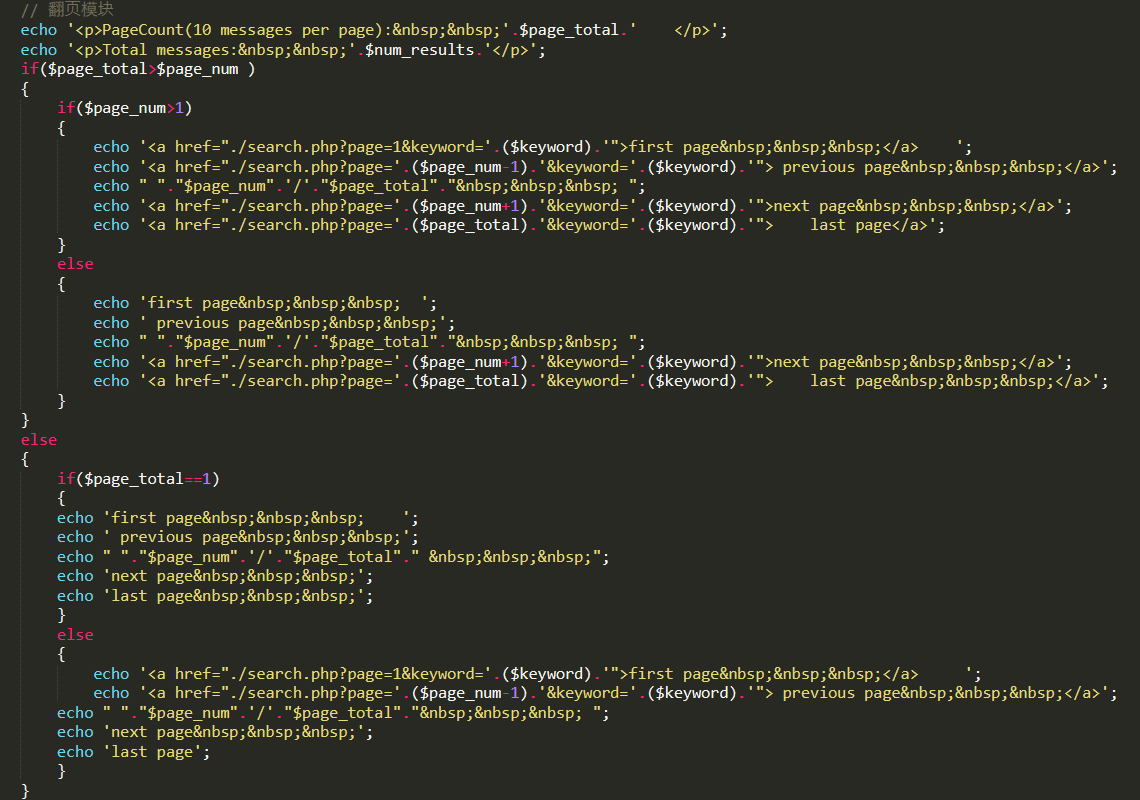
\includegraphics[scale=0.3]{img/dsw_chao.png}
\caption{Hyperlinks}
\label{fig:dsw2}
\end{figure}

When setting the hyperlinks, what matters is that we should send the parameter 'keyword' besides the parameter 'page'. Another important thing is that sometimes some hyperlinks needn't be use. For example, if we are at the first page, the hyperlinks of the statement 'first page' is unnecessary.So we should write some specific 'if' statement to judge if we should use the hyperlinks.
(See \ref{fig:dsw2} on the next Page)

\begin{figure}[H]
\centering
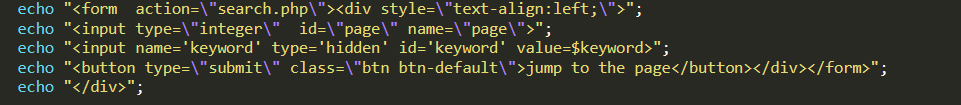
\includegraphics[scale=0.35]{img/dsw_input.png}
\caption{Paper Jumping}
\end{figure}

When it comes to the page jumping, what should be mentioned is that to reduce the error such as the number user entered is out of the limitation of the actual pages, we let the actual page you jump to is always the last page if you input a number that is greater than the number of total pages.

\subsection{Demonstration}
An example is demonstrated as follows.
\begin{figure}[H]
\centering
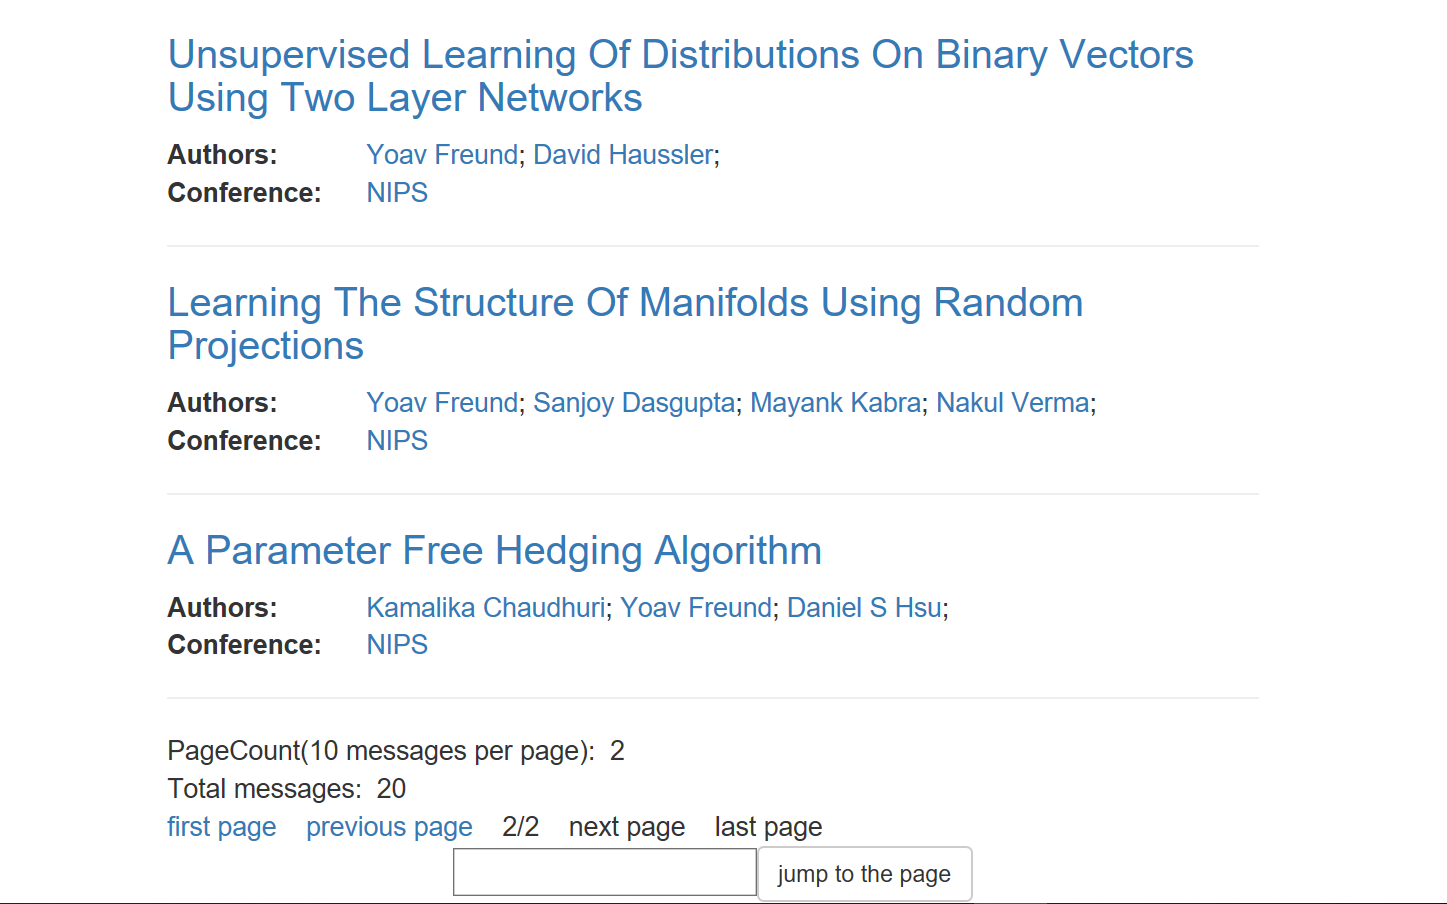
\includegraphics[scale=0.15]{img/dsw_ex.png}
\caption{AUTHOR EXAMPLE}
\end{figure}
This is the last page of the author page.

\section{Version II: by jQuery}
In the first version of paging design, only PHP code is used, and the use of the 'Page' parameter means that the page would be reloaded every time the page was turned. Obviously, all that needs to be refreshed is the table that shows the data, and the rest of the page will remain unchanged. If we can only refresh the data table every time you turn the page, and keep the other parts unchanged, then we can further improve the efficiency of the web page. 

With this idea in mind, we started the second version of page turning design.

\subsection{Description}
First, let's show the second version's page turning . We take the search results on the'search'page as an example, and the effect is shown in the following figure.

Ten pieces of information are displayed on each page. At the bottom of each page, the number of the current page and total pages can be displayed. By clicking the'previous'and'next' buttons, the page can be turned up and down. By clicking the'first'and'next' buttons, the page can be turned to the first and last pages. In addition, we can also click the button corresponding to the page numbers before or after the current page with a total of five pages.

\begin{figure}[H]
\centering

\includegraphics[scale=0.25]{img/dsw_1.png}

\end{figure}



Because of the use of'jQuery'to achieve page turning , after a load, we can quickly change the page without refreshing, and after the page is turned, we still stay in the previous position, instead of moving back to the top of the page, which makes the page turning function more convenient and fast.

\subsection{Solution}

Unlike the first version where the search scope is determined according to the'page' parameter and each time we don't search all data, in this version, we can search all the results at one time and divide them into many parts. Each page turn shows the information of one part and hides the information of the rest. That is to say, we can divide the searched information into different'divs', add page turning function on the button, and change the display style of different divs when clicking.

Similarly, we can divide the buttons corresponding to different page numbers into many divs, hide part and display part when clicking, and then we can achieve the page turning without refreshing.


\subsection{Source Codes}
Now we still take the search page as an example to present the page turning.

\begin{figure}[H]
\centering
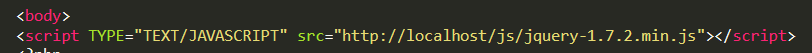
\includegraphics[scale = 0.35]{img/dsw_2.png}
\caption{Premise}
\end{figure}

At the beginning, we should import the 'jquery'. The codes are shown in the figure 'premise'.


\begin{figure}[H]
\centering
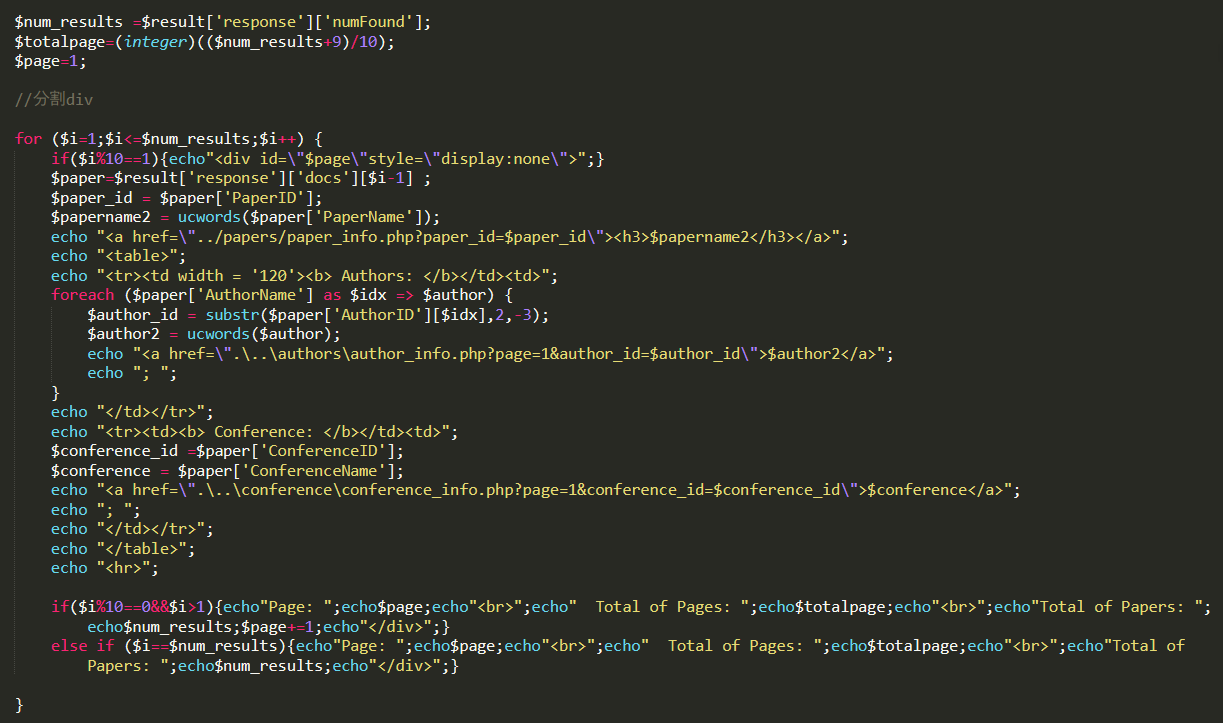
\includegraphics[height=6.0cm,width=10.0cm]{img/dsw_divide.png}
\caption{Dividing divs}
\end{figure}




Before we divide all information into different divs, we should know the number of total information we get and figure out the number of total pages which depends on how many pieces of data we want to show in a page. Then we use 'for' circle statement to divide the data into many divs. Every div's
style is set as 'hidden' at first by using the statement 'display:none'. And at the end of each div, we show the number of total pages and the current page.The codes are shown in the figure'Dividing divs'


\begin{figure}[H]
\centering
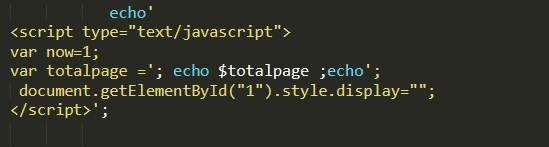
\includegraphics[width=6.0cm]{img/dsw_3.png}
\caption{Start}
\end{figure}

The codes in the figure 'Start' are to send the variable 'page' to the javascript and change the first page's display style from hidden into shown.

\begin{figure}[H]
\centering
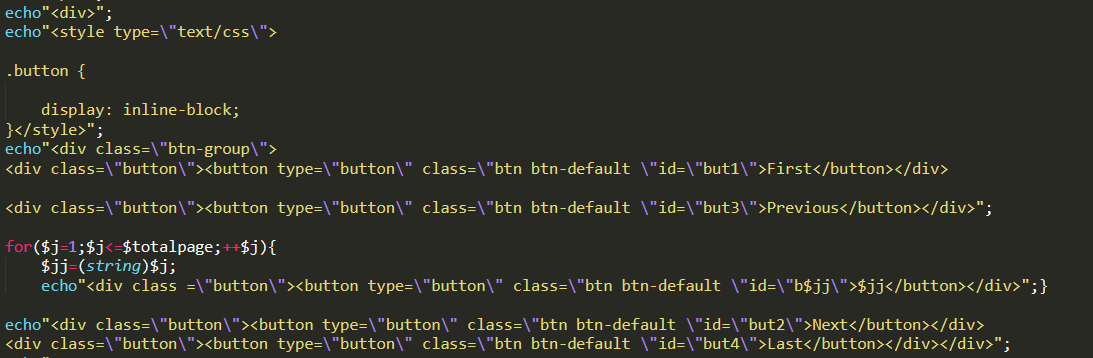
\includegraphics[width=11.0cm]{img/dsw_button.png}
\caption{Buttons}
\end{figure}


Then as the figure 'Buttons' shows, we create four buttons 'first','previous','next' and 'last' which are used to realize the primary function of page turning. Then we create a corresponding button for each div, all of which are in the different divs, whose display style can also be changed by clicking. To make them look neater, we set their display style as 'inline block', which make sure that all buttons are shown in one line.

\begin{figure}[htbp]
\centering
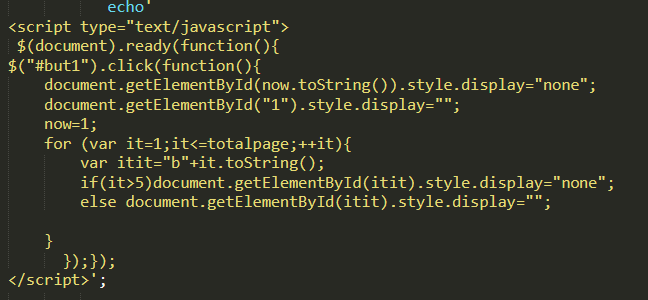
\includegraphics[width=7.0cm]{img/dsw_first1.png}
\caption{First Button}
\end{figure}

\begin{figure}[htbp]
\centering
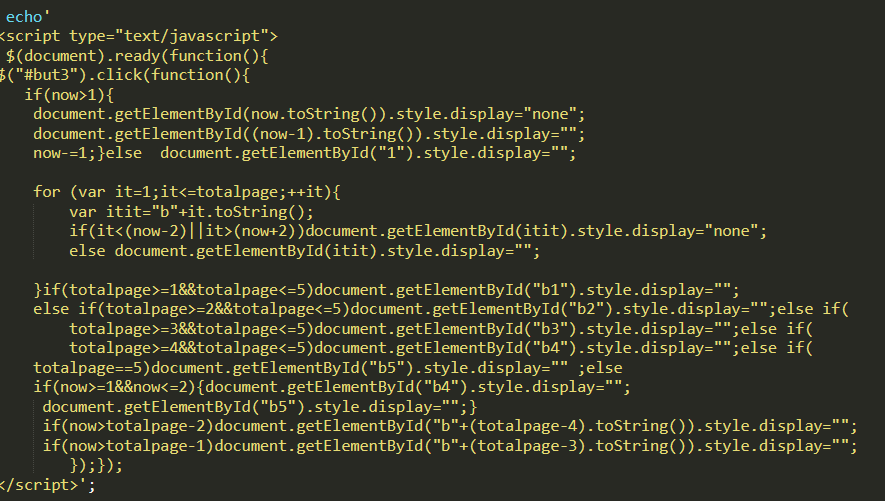
\includegraphics[width=7.0cm]{img/dsw_pr1.png}
\caption{Previous Button}
\end{figure}

\begin{figure}[htbp]
\centering
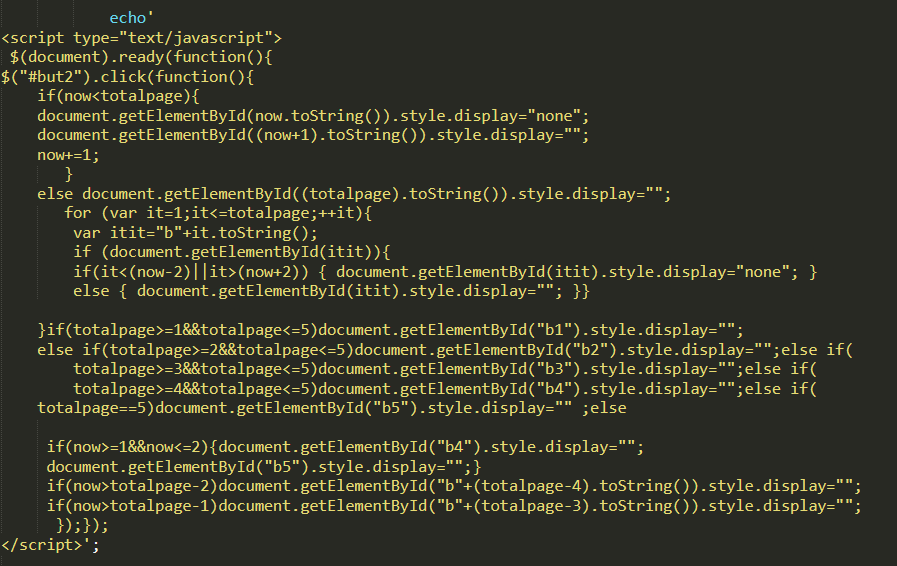
\includegraphics[width=7.0cm]{img/dsw_next1.png}
\caption{Next Button}
\end{figure}

\begin{figure}[htbp]
\centering
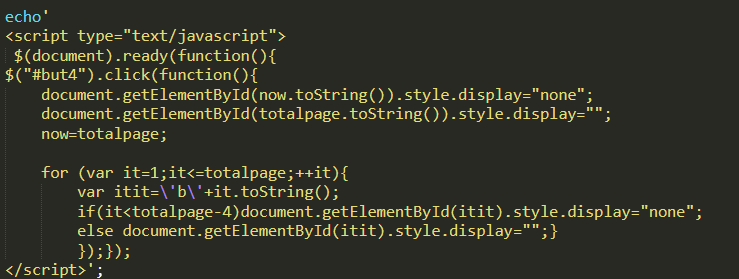
\includegraphics[width=7.0cm]{img/dsw_last1.png}
\caption{Last Button}
\end{figure}

\begin{figure}[htbp]
\centering
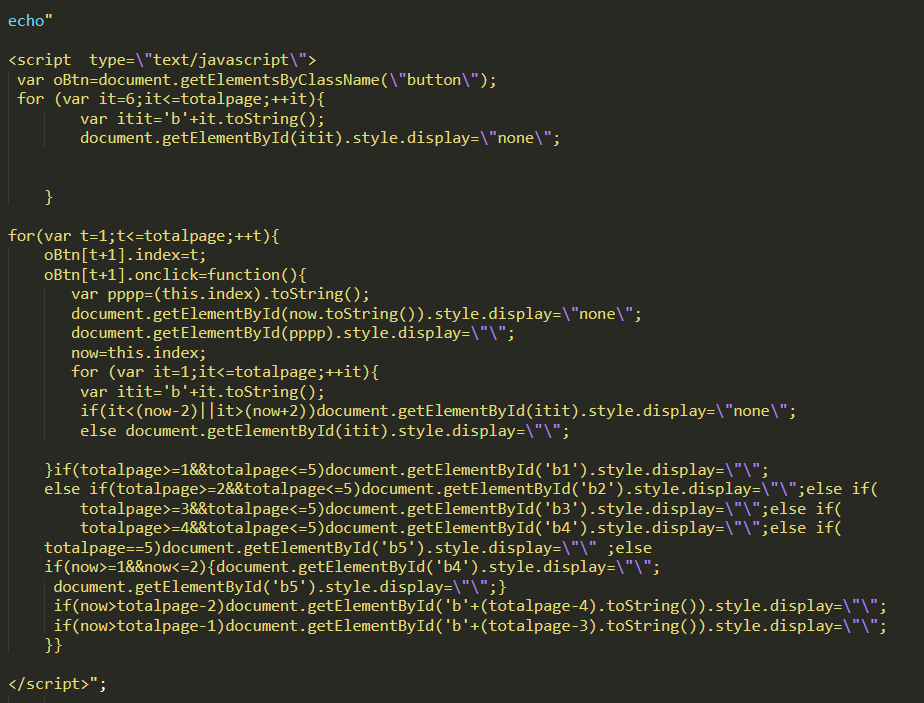
\includegraphics[width=10.0cm]{img/dsw_fun.png}
\caption{Button function}
\end{figure}

Now we should set function for the buttons.In each button's function, we decide which divs should be shown and which divs should be hidden by the current page number. And we can change their display style by their div's id using the statement 'document.getElementById('b4').style.display='. Similarly, we also need to show or hide the buttons of each page. What should be mentioned is that when the total number of pages is less than 5, the function of pages' buttons' display should be write in different ways.





\subsection{Demonstration}
Some examples are demonstrated as follows.

Figure \ref{pict:dsw1} shows the first page of an author.

Figure \ref{pict:dsw2} shows the last page of a conference.

\begin{figure}[b]
\centering
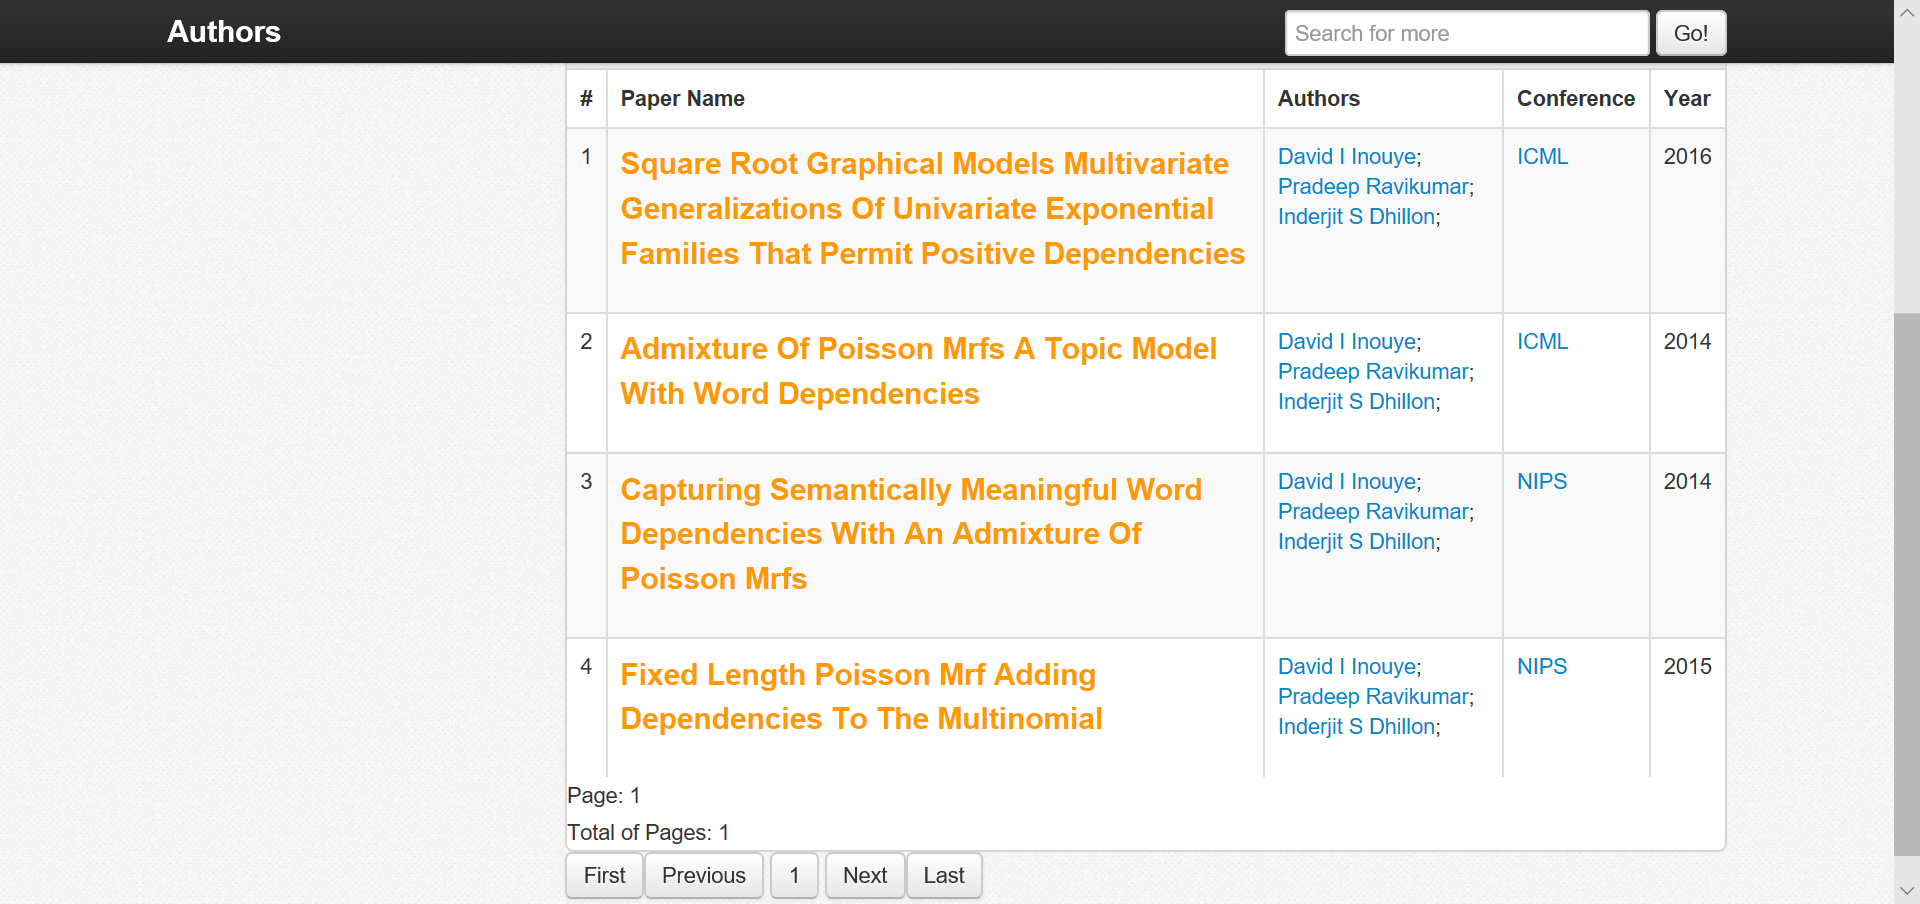
\includegraphics[width=11.0cm]{img/dsw_author.png}
\caption{AUTHOR EXAMPLE}
\label{pict:dsw1}
\end{figure}

\begin{figure}[b]
\centering
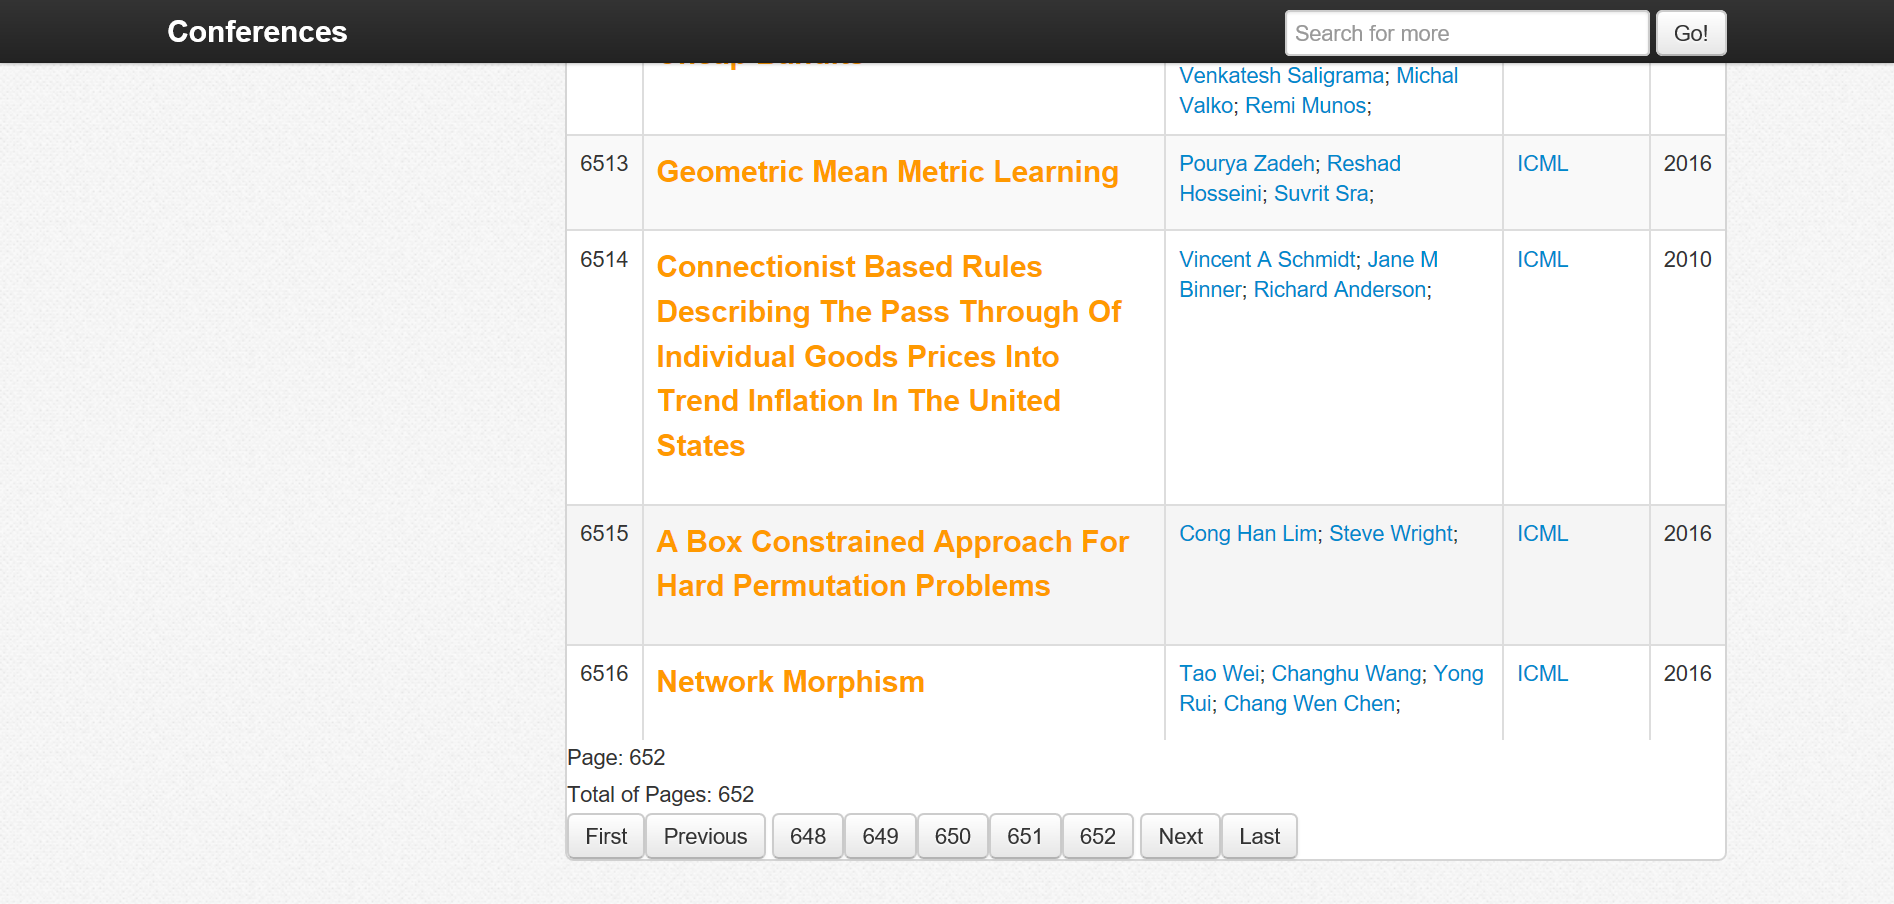
\includegraphics[width=11.0cm]{img/dsw_con.png}
\caption{AUTHOR EXAMPLE}
\label{pict:dsw2}
\end{figure}




\chapter {Integrated Searching Bar}

We use the copy field in solr to realize an integrated searching bar. By making copies of fields to one field, we can apply several distinct field types to a single piece of incoming information.

To construct a copy field, we first add a new field, for example a field 'keyword'. Then we choose ``keyword'' as destination and 'AuthorName', 'ConferenceName' and 'PaperName' as sources. Now, a query to 'keyword' can search all related information in three fields. In this way, we only need one integrated searching bar and do the query for one time to get all reults.


\chapter {Data Visualization}


\section {Statistical Graph}
In our website, we have 12 charts made by echarts altogether to visualize the data in the form of 3D histogram, pie chart, line chart and bar chart.

\subsection {3D histogram}

\begin{figure}[H]
\centering
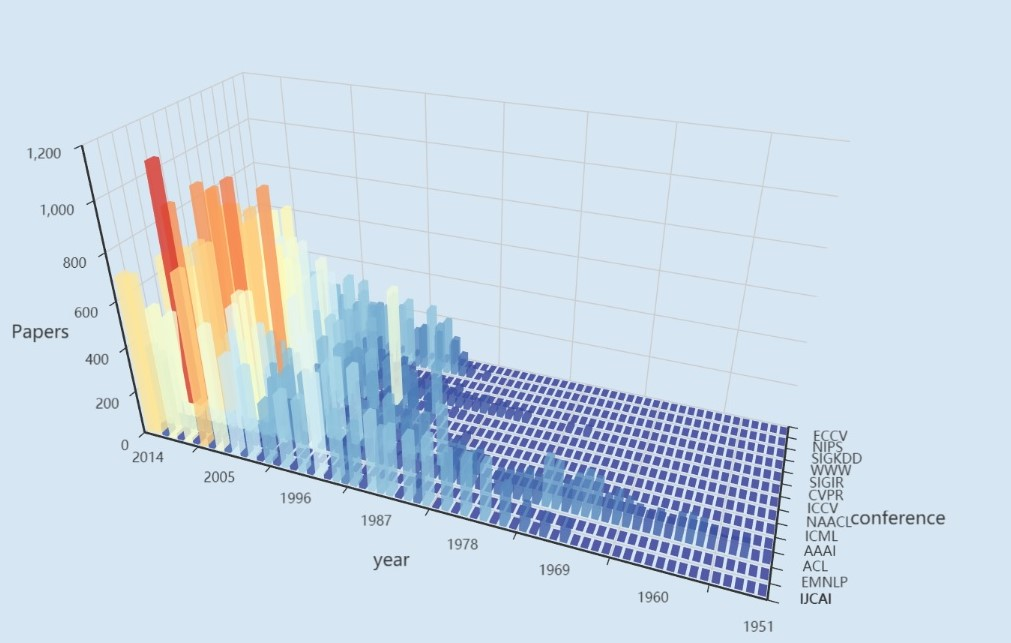
\includegraphics[scale=0.55]{img/fsh_3d_hist.jpg}
\caption{3D chart in the homepage}
\end{figure}

In the homepage, we have a 3D chart to show the publication tendency of every conferences. This is a static chart that we prepare the data in advance. To construct a 3D chart in echarts, we need an array that concludes three-dimension coordinates. The z-axis value refers to the publication.

\begin{figure}[H]
\centering
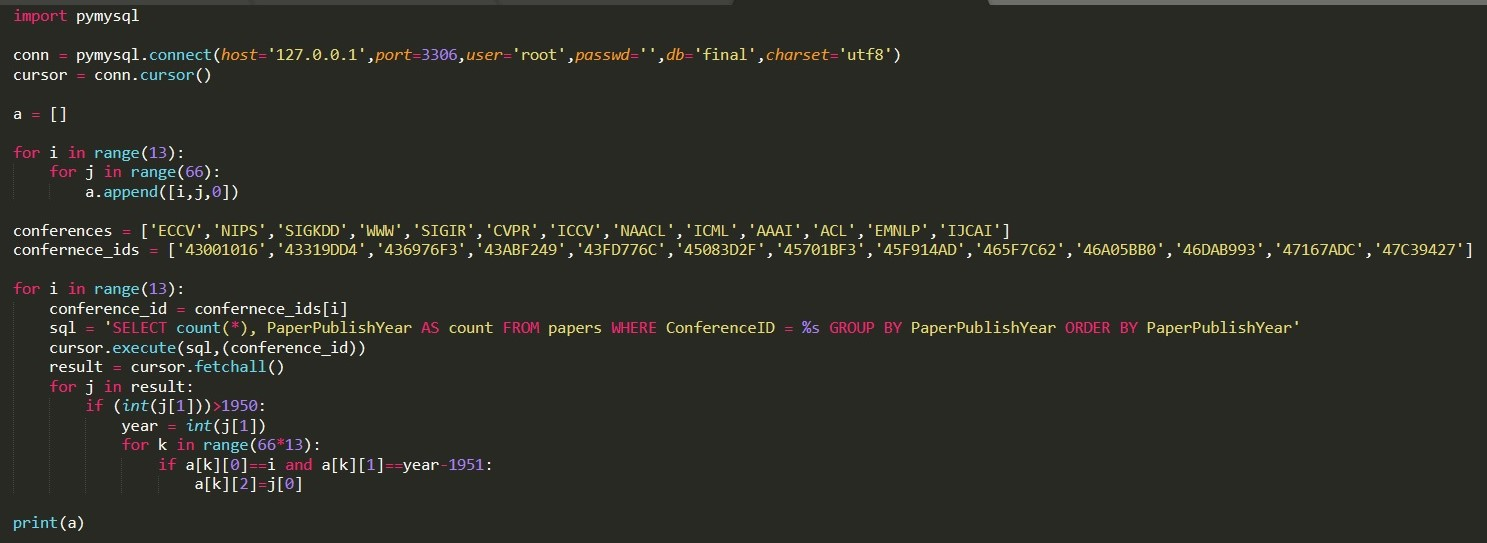
\includegraphics[scale=0.45]{img/fsh_code_1.jpg}
\caption{Get data form Mysql}
\end{figure}

\subsection {Bar chart, pie chart and line chart}

The codes are similar when we construct a bar chart, pie chart or line chart. We need two arrays to show the x-axis coordinates and their values. We first get the data from Mysql database and then convert the php array to javascript. SQL languages 'GROUP BY' and 'count(*)' are massively used to get the data.
\par The following three charts come from conference page, search page and author page respectively. All codes related to these charts are in file 'pages / XX / XX \_charts.php'.
\par It's worth mentioning that to make all charts intelligible, we need to adjust the parameters in echarts option. For example, we set 'yAxis.minInterval: 1' so that decimal won't appear in y-axis labels. Also, we set 'xAxis.axisLabel.rotate: 40' so that all labels can all labels can be displayed(See Figure \ref{fig:bar chart example}).

\begin{figure}[H]
\centering
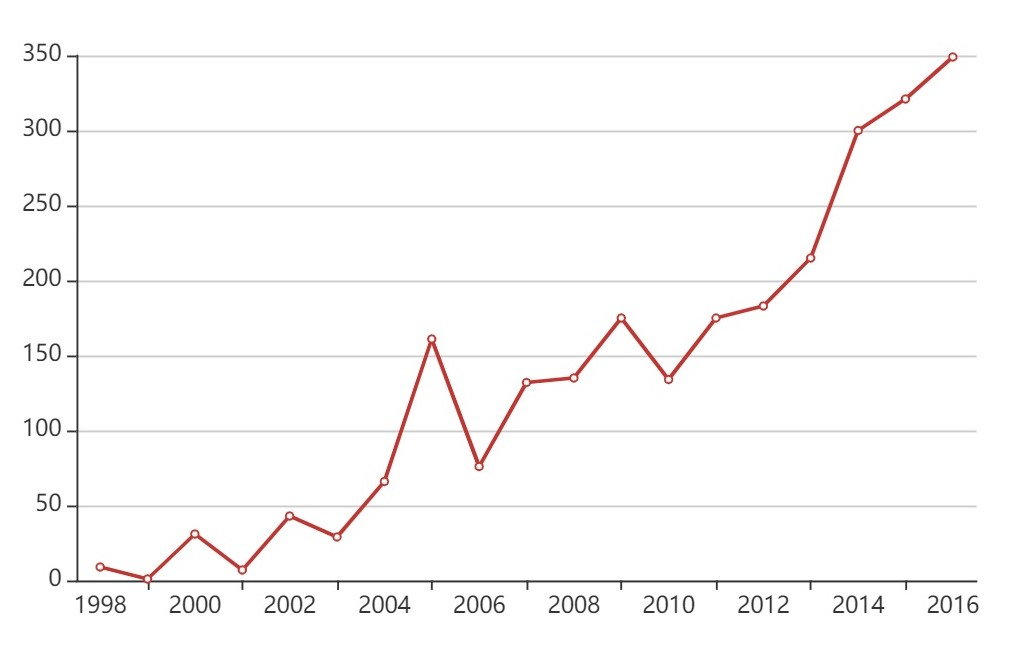
\includegraphics[scale=0.6]{img/fsh_line.jpg}
\caption{Line chart example}
\end{figure}

\begin{figure}[H]
\centering
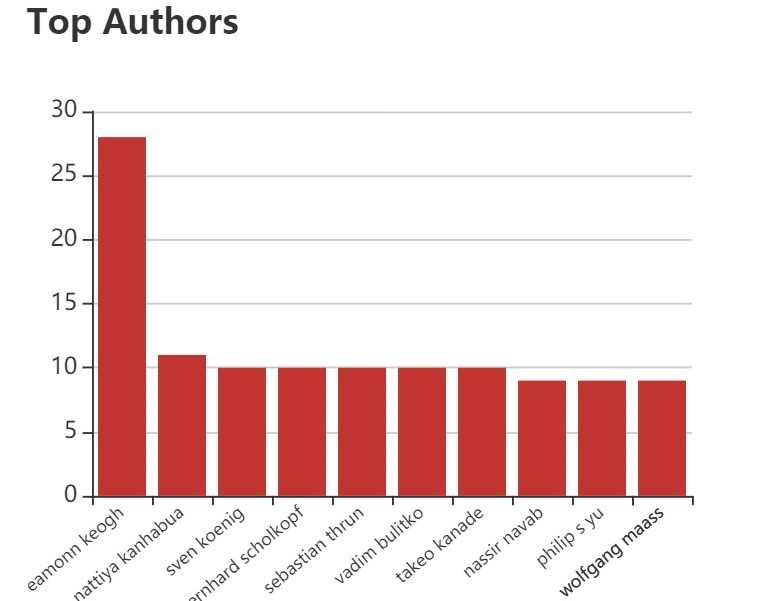
\includegraphics[scale=0.7]{img/fsh_bar.jpg}
\caption{Bar chart example}
\label{fig:bar chart example}
\end{figure}

\begin{figure}[H]
\centering
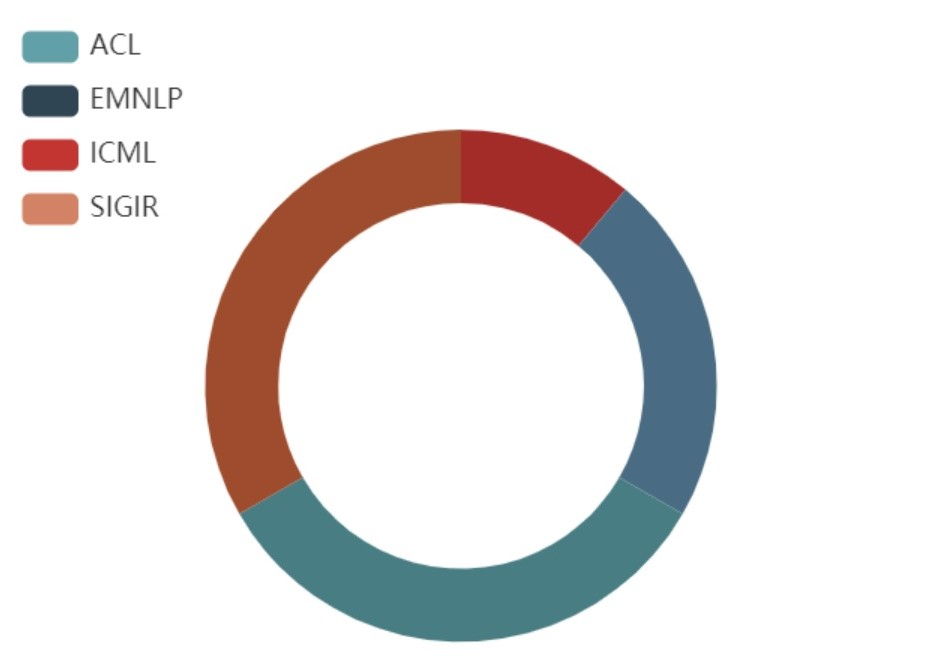
\includegraphics[scale=0.7]{img/fsh_pie.jpg}
\caption{Pie chart example}
\end{figure}



\section {Paper Relation Graph}

A relation graph can visually reveal the relationship between papers, which we believe will be of great help to the users. For every paper, we've prepared a relation graph to show its reference papers, and the reference papers of its reference papers. Visitors can have a clear picture of how the paper is derived by looking at multiple levels of reference papers.

\subsection{Description}

We've applied a built-in template in echarts when making the relation graph. First we've fetched all the paper\_reference relationship concerned, including multiple levels of reference relations, from the database. Then based on these data, we translate them into two arrays, namely nodes and links, which can be accepted by the echarts template. In the meantime, we add more information such as paper title, weight of the nodes and styles of the links into the array. Then the relation chart can be generated by echarts. In addition, we also wrote a jQuery function by ourselves in order to allow our users to visit the cited paper directly by clicking the nodes or the links. Some demo screenshots are listed below.

\begin{figure}[htp]
\centering
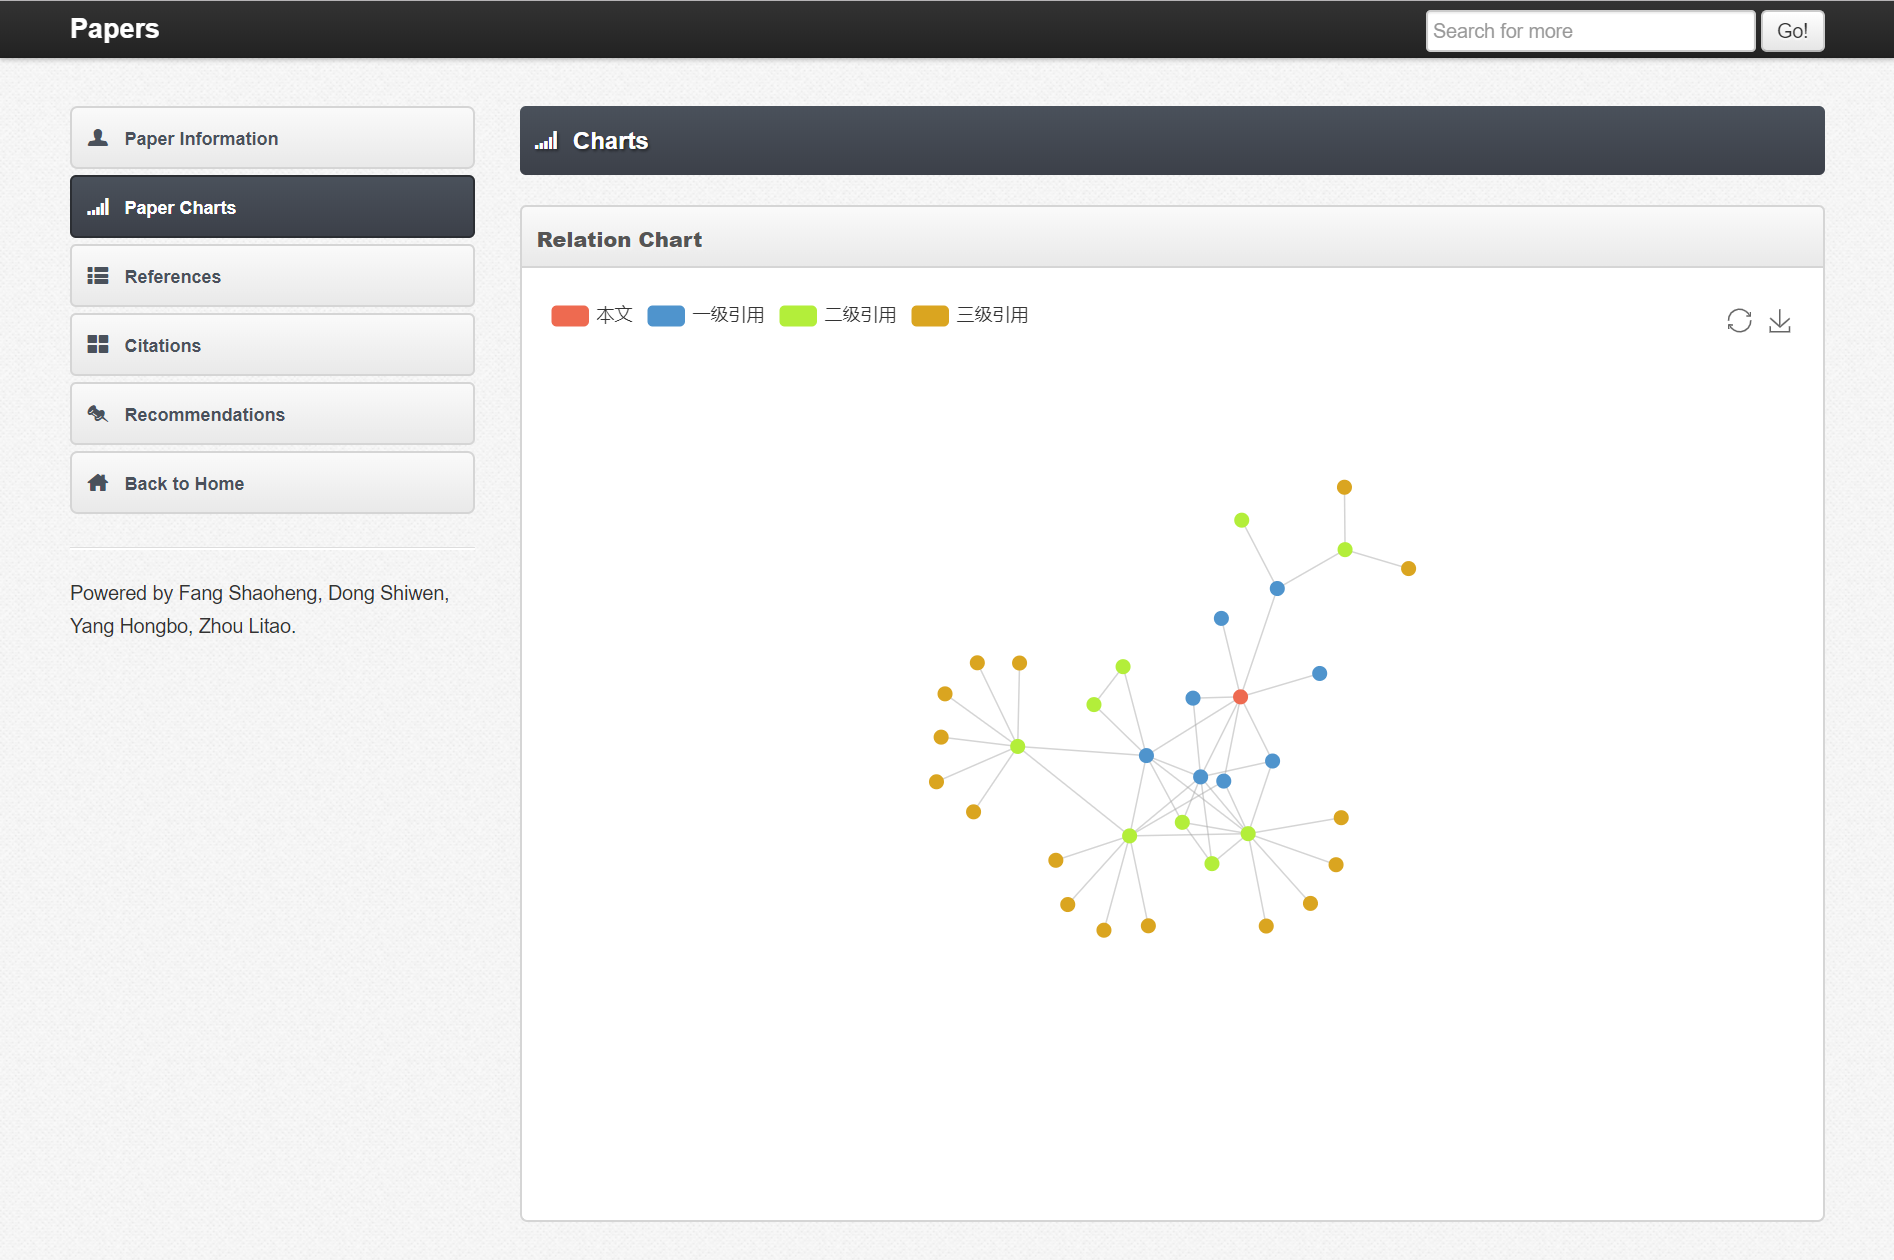
\includegraphics[width=11cm]{img/zlt_rel_demo.png}
\caption{Relation Chart Page}
\end{figure}

\begin{figure}[htp]
\centering
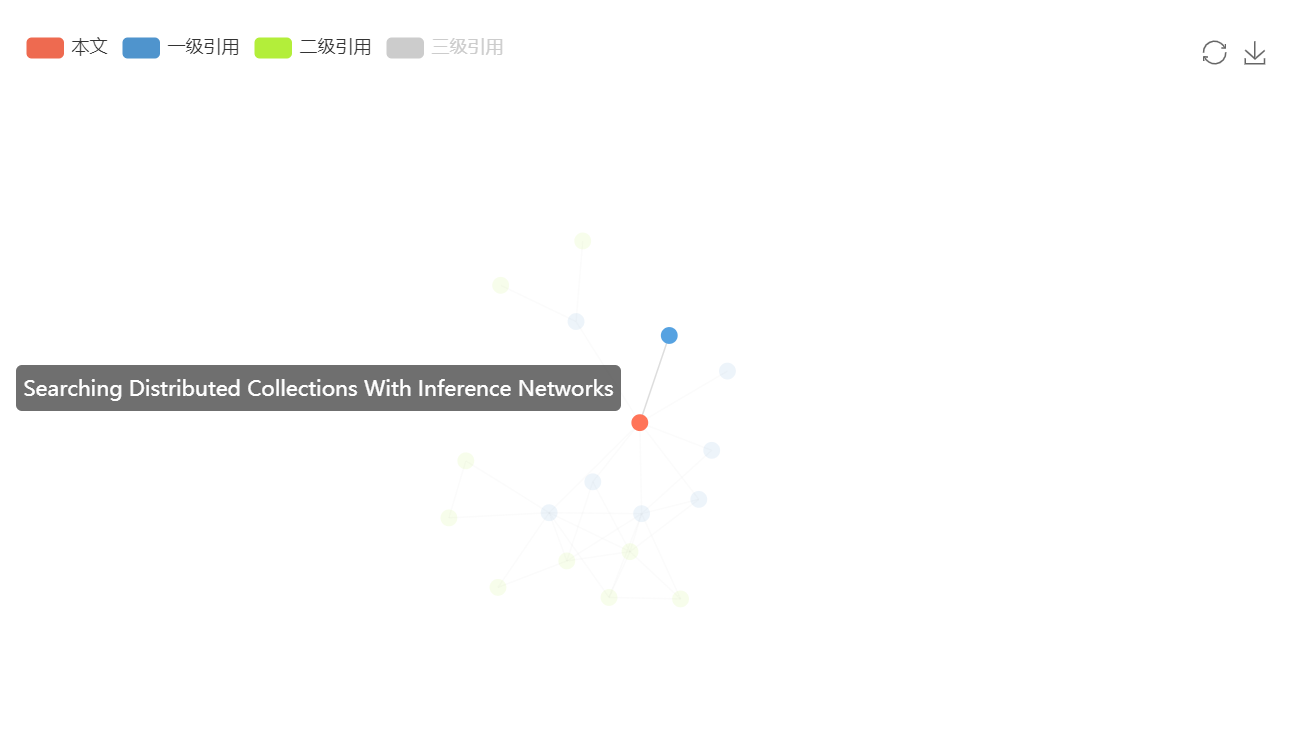
\includegraphics[scale=0.3]{img/zlt_rel_demo1.png}
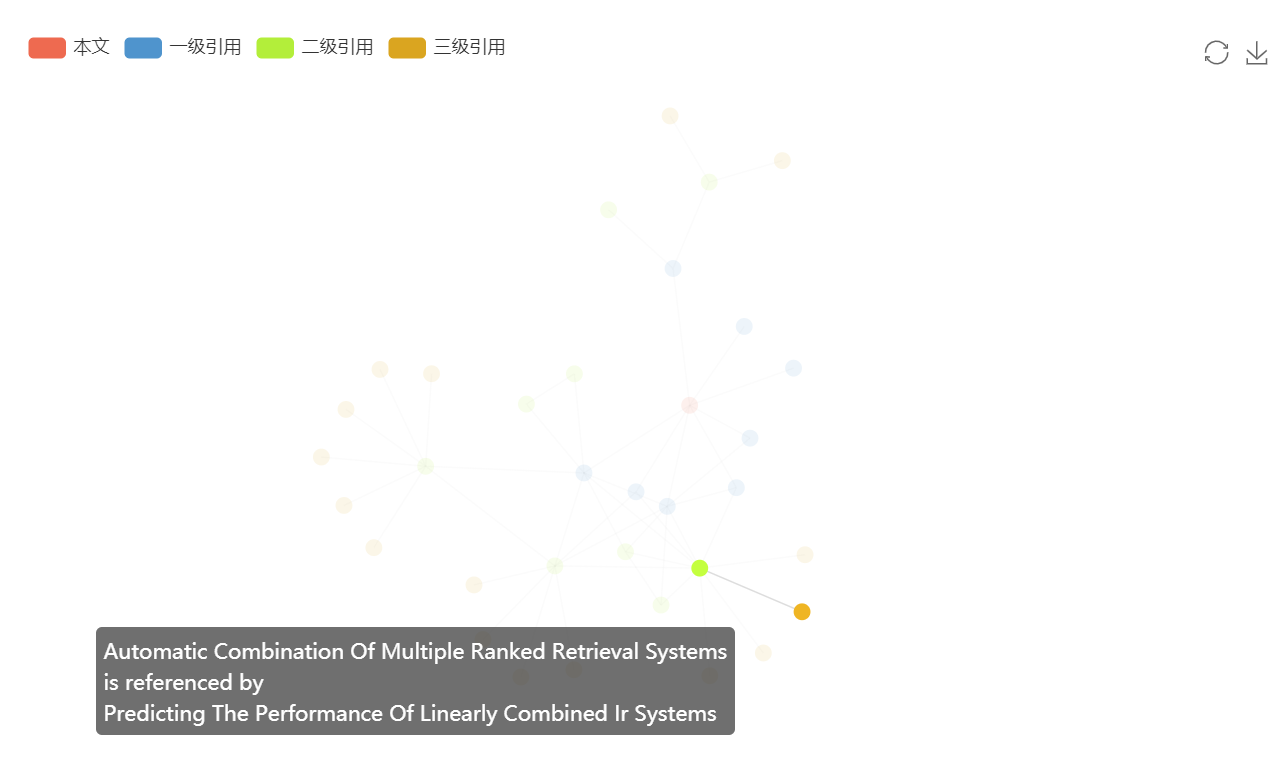
\includegraphics[scale=0.3]{img/zlt_rel_demo2.png}
\includegraphics[scale=0.3]{img/zlt_rel_demo3.png}
\caption{Multiple Display Modes \& functions}
\end{figure}

\subsection{Collect the Data}

For convenience's sake, we first wrote a function in order to integrate the search of a paper's name into a function call. The ucwords() is a useful function in PHP, which can turn the first letter of every word into upper case. This can give our information display a better look.

\begin{figure}[htp]
\centering
\includegraphics[scale=0.55]{img/zlt_rel_code_func.png}
\caption{get\_paper\_name function}
\end{figure}

Then we use MySQL to get the direct reference of the paper. For these referenceIDs, we wrote a loop to add them to the nodes array, and put these first-level relations directly into the links array.

\begin{figure}[htp]
\centering
\includegraphics[scale=0.55]{img/zlt_rel_code_lev1.png}
\caption{First Level Data Collection}
\end{figure}

After that, we wrote a nested loop. The first level is to loop through the depth (i.e. the reference level), the second level is to loop through reference papers of the last reference item. The searching structure is just like building a tree. Note that we've created a helping array storing the paperids that we've already added into the nodes array, so that we can avoid overlapping nodes. Theoretically, the reference level (depth) can be streatched to infinity, but for practical use, we assume the depth of 4 will be fine. (See Figure \ref{fig:rel_high} on next Page)

\begin{figure}[htp]
\centering
\includegraphics[scale=0.55]{img/zlt_rel_code_lev2.png}
\caption{Higher-Level Data Collection}
\label{fig:rel_high}
\end{figure}


\subsection{Set Echarts Options}

The links and nodes arrays we've created above are just what the built-in echarts template requires. However, the initial graph configurations were not suitable for our information. (See Figure \ref{fig:rel_contrast} on next Page) We need to block the display of node ids and loosen the distance between dinstinct nodes. After some manual regulating work, we make the graph look a lot better. Our major configuration codes are listed below. (See Figure \ref{fig:rel_codess} on next Page)

\begin{figure}[htp]
\centering
\includegraphics[scale=0.55]{img/zlt_rel_demo4.png}
\includegraphics[scale=0.55]{img/zlt_rel_demo5.png}
\caption{A Contrast between the Original and the Present Version of Paper Relation Charts}
\label{fig:rel_contrast}
\end{figure}

\begin{figure}[htp]
\centering
\includegraphics[scale=0.55]{img/zlt_rel_code_config.png}
\caption{Echarts Options Configuration}
\label{fig:rel_codess}
\end{figure}

\subsection{Node Labels}

The labels of our nodes should show the paper's name and the labels of our links should show the name of the two papers in the reference relation. This work has already been finished when we are collecting the data. We set the label of the nodes to be exactly what we want to show to our users. A further step we took is to add hyper-links to every nodes and edges. Note that the name of every node is its PaperID, which can be directly applied to the URL, while the name of every link is composed of the reference node and the origin node. We use the string carving function in PHP to get the first 8 character, representing the reference node, so users can access the reference page by clicking the links.

\begin{figure}[htp]
\centering
\includegraphics[scale=0.55]{img/zlt_rel_code_label.png}
\caption{Create Hyper-links for Node Labels}
\end{figure}


\section{Big Charts using Gephi}

As the saying goes, ``One picture worths 1000 words.'', a visualization picture is vital to show the connection between objects in some scales. To show an overall relationship, we choose  \textbf{gephi} to visualize the data collected by MySQL. This method can help the part of E-charts to draw a better pictue in users' mind. 
There was a problem that troubled us for a long time. That is: how can we put the picture onto the pages. And it is finally solved by using package ``ariutta/svg-pan-zoom
'' from GitHub. 
Here we'll give MySQL sequences and the way to draw a gephi picture(.svg).

\subsection{MySQL Fetch}

We choose to show the connection between authors in all 13 conferences. We established the connection by reference and citation. And this demands us to use `join search' in MySQL. Example codes are given below.(We take ConferenceID= `47c39427' for an example.)

\begin{figure}[H]
\centering
\includegraphics[width=11cm]{img/yhb_my_1.png}
\caption{search example}
\end{figure}

Finally, remember to lead the data out in (.csv) format, in order that we can use the data in gephi easily.

\subsection{Gephi Drawing}

Gephi can use data in (.csv) format directly. After transmitting information into gephi, we can find a picture in the window. But this picture is so ugly and unclear that we cannot take it for visualization use derectly.  

\begin{figure}[H]
\centering
\includegraphics[width=11.0cm]{img/yhb_ge_1.png}
\caption{geghi: original picture}
\end{figure}
We may turn to gragh-drawing methods such as ``force directed method'' and ``Fruchterman Reingold method'', to better display the characteristics of the relationship between authors.

Next, we can adjust the  size of each node by degree, and give them different colors.
It's much easier for us to see the relation.
\begin{figure}[H]
\centering
\includegraphics[width=11.0cm]{img/yhb_ge_2.png}
\caption{geghi: processed picture}
\end{figure}
Finally, we can transmit it as (.svg) file to load on the pages.

\chapter {Beautify the Pages}


\section {Index Beautification}

There are altogether four parts in the index page: the top banner, the search box part, a chart and the bottom banner. The introduction of the chart is in the data visualization chapter.

\begin{figure}[H]
\centering
\includegraphics[scale=0.4]{img/fsh_index.jpg}
\caption{The index page}
\end{figure}

\subsection {Top banner}

In the top banner, we have our website's name 'Smart Boy' and two buttons, 'search' and 'chart'. By clicking the button, the page will jump to the search part or the chart part.


We use 'navbar' in bootstrap to complete out top banner. The links of 'search' and 'chart' are written in the nav tag(See in Figure \ref{fsh code 1}).

\begin{figure}[H]
\centering
\includegraphics[scale=0.6]{img/fsh_index_tp.jpg}
\caption{The top banner in index page}
\end{figure}


\begin{figure}[H]
\centering
\includegraphics[scale=0.6]{img/fsh_index_code_1.jpg}
\caption{Codes of the top banner}
\label{fsh code 1}
\end{figure}

\subsection {Search box \& main part}

\begin{figure}[H]
\centering
\includegraphics[scale=0.45]{img/fsh_index_sb.jpg}
\caption{The search box in index page}
\end{figure}

\begin{figure}[H]
\centering
\includegraphics[scale=0.45]{img/fsh_index_code_2.jpg}
\caption{Codes of the search box}
\end{figure}


First, we use bootstrap animation 'probootstrap-animate' to make all contents display gradually.
\par We also use 'placeholder' in the input tag to show sentence in the searching box

\subsection {Bottom banner}

At the bottom of the index page, we show some basic information of our website. We also have a link connected to our lesson website.

\begin{figure}[H]
\centering
\includegraphics[scale=0.45]{img/fsh_index_bottom.jpg}
\caption{The bottom banner in index page}
\end{figure}


\section {Pages Beautification}

Our original page styles were derived from LAB3, which were very basic. With more and more functions implemented, we found that one page was not enough to carry all the information. As a result, we decided to split one page into several subpages carrying out different functions. For example, we split the paper.php page into information page, charts page, reference page, citation page and recommendation page. With the help of online resources, we fit our contents into a well-defined template. (tribute to http://www.cssmoban.com)


\begin{figure}[H]
\centering{}
\includegraphics[scale=0.35]{img/zlt_beau_demo.png}
\caption{General Structure of the Pages}
\end{figure}

As the screenshot above reveals, all the pages share a similar layout - a top banner containing the page title and a small search bar, a right navigating column linked to all the related pages in this section and the right division where the main contents of the page are located.

\subsection {Top Banner \& Small Search Bar}

Our template was originally designed for backstage admin system. In order to better fit our webpages, we replace the user login button with a small search bar. The search bar was a simple ``form'' application, but it turned out to be very useful when we are testing and using our pages. Codes of this part are listed as follows.

\begin{figure}[H]
\centering{}
\includegraphics[scale=0.35]{img/zlt_beau_codes.png}
\caption{Top Banner}
\end{figure}


\subsection {Left Navigation Bar}

The template has already provided a series of button icons (derived from bootstrap framework) and a well-formatted list of buttons. To make our own navigation bar, we just need to change the icons according to the given names, and get the name and hyper-links right. Also, we can specify the class to be ``active'' in order to highlighten the button representing the current page.

\begin{figure}[H]
\centering{}
\includegraphics[scale=0.35]{img/zlt_beau_bar1.png}
\includegraphics[scale=0.35]{img/zlt_beau_bar2.png}
\caption{Left Navigation Bar}
\end{figure}

\subsection {Main Contents}

Since the template is based on the framework of Bootstrap, in the main contents, it follows that we should obey the rules of Bootstrap, such as containers, row classes, and the twelve column layout. Take a particular page for example, the generating process of the table through PHP is omitted. The layout for other pages are simlar in principle.
\begin{figure}[H]
\centering{}
\includegraphics[scale=0.35]{img/zlt_beau_cont1.png}
\includegraphics[scale=0.35]{img/zlt_beau_cont2.png}
\caption{Main Contents}
\end{figure}



\chapter {MySQL Optimization in Affiliation Pages}

The affiliation section is a section all made by ourselves. However, as has been briefly introduced in the Affiliation Pages section, new problems arise that the loading speed is too slow. This is because in our solution, the big paper\_author\_affiliation table will be searched everytime we display a new row in the webpage, which is clearly unnecessary. (See Figure \ref{fig:opt_basic})
{}
\begin{figure}[H]
\centering{}
\includegraphics[scale=0.45]{img/zlt_opt_code_basic.png}
\caption{Base Version in Affiliation Pages}
\label{fig:opt_basic}
\end{figure}


\section {Solution}
Through practice, we found that the main factor dragging the loading time slow is the call by PHP for MySQL query. In order to reduce the loading time, we need to control the time we call a MySQL query. However, generally speaking, since we first need to get the authors based on the affiliation\_id, and then find the detail information based on the author we have found in the first query, there is an unavoidable iterating structure in the process. The solution to this problem is not as easy as we assumed.

Eventually, we came up with the idea that all the searching work with MySQL can be integrated into one query. And we may just select the information we need from the total query results in order to display the information in the pages. This solution has restricted the searching query call to one single time. However, this will creat some difficulty when we want to echo the information onto the webpage.

\section {Integrated MySQL Query in Authors List}

Instead of searching the author information piece by piece, the searching query we write (See Figure \ref{fig:opt_query}) will return a group of rows showing the paper / affiliation information about one single author.

The basic idea about this integrated query is join the paper\_author\_affiliation table to itself, with restricting conditions of course. Our final result is a simplified paper\_author\_affiliation table, containing the author directly linked to the affiliaiton and the papers which might not be published in this affiliation, but whose authors once belonged to the affiliation. With the GROUP BY technique, the rows of every author can be returned group by group.

\begin{figure}[H]
\centering
\includegraphics[scale=0.55]{img/zlt_opt_code_query.png}
\includegraphics[scale=0.55]{img/zlt_opt_code_queryres.png}
\caption{Integrated MySQL Query}
\label{fig:opt_query}
\end{figure}

\section{Echoing Tricks in Authors List}

Unlike what we did in the base version, where MySQL queries and PHP iterative loops are mixed together in an intuitive structure, here we are looping through the rows in the integrated searching results. (See Figure \ref{fig:opt_query}) So in every loop, we need to first judge whether this row is talking about the same author above or it starts a new one. Within the group corresponding to the same author, we just add one more affiliation into the webpage (before that we have to judge whether the affiliation is a new one, of course). While if the row marked the start of a new author, we have to end the previous row, begin a new row on the webpage. With these tricks, the final outlook on the webpage is just the same as the base version, but boasts a loading time within a second. The main part of the codes are listed below. (Initialization and Clean-up work omitted) The same tricks also apply to Paper List on the affiliation\_paper page. 


\begin{figure}[H]
\centering{}
\includegraphics[scale=0.45]{img/zlt_opt_code_advanced.png}
\caption{Echoing Tricks}
\end{figure}

\section{Integrated MySQL Query in Top Authors Charts}

As has been discussed before in the Charts section, the top author charts require a list of author names and a list of numbers representing their publications counts. The same problem occurs that the data collecting work was taking too much time. We are also using MySQL joint search to replace PHP loops. We use count (DISTINCT ) + GROUP BY commands to directly get the result. The MySQL queries are listed below. Further processing on the searching results are fragile and hence omitted. 

\begin{figure}[H]
\centering{}
\includegraphics[scale=0.55]{img/zlt_opt_code_chart.png}
\caption{Integrated MySQL Query in Top Authors Charts}
\end{figure}

All the three parts introduced above make up our optimization of the affiliation section.


\backmatter

\chapter {Appendix}

\section*{Division of Writing}

\begin{table}[H]
\begin{tabular}{lll}
\hline
\textbf{Chapter}                             & \textbf{Section}             & \textbf{Writer}        \\ \hline
\multicolumn{2}{l}{\textbf{Preface}}                                        & \textit{Litao Zhou}    \\
\multirow{2}{*}{\textbf{I. Enrich Contents}} & Paper \& Conference Pages    & \textit{Hongbo Yang}   \\
                                             & Affiliation Pages            & \textit{Litao Zhou}    \\
\multirow{2}{*}{\textbf{II. Leaf Turning}}   & Version I: by PHP parameters & \textit{Shiwen Dong}   \\
                                             & Version II: by jQuery        & \textit{Shiwen Dong}   \\
\multicolumn{2}{l}{\textbf{III. Integrated Search Bar}}                     & \textit{Shaoheng Fang} \\
\multirow{3}{*}{\textbf{IV. Visualization}}  & Statistical Graph            & \textit{Shaoheng Fang} \\
                                             & Paper Relation Graph         & \textit{Litao Zhou}    \\
                                             & Big Charts using Gephi       & \textit{Hongbo Yang}   \\
\multirow{2}{*}{\textbf{V. Beautify Pages}}  & Index Beautification         & \textit{Shaoheng Fang} \\
                                             & Pages Beautification         & \textit{Litao Zhou}    \\
\multicolumn{2}{l}{\textbf{VI. MySQL Optimization in Affiliation Pages}}    & \textit{Litao Zhou}    \\
\multicolumn{2}{l}{\textbf{Conclusion}}                                     & \textit{Litao Zhou}    \\ \hline
\end{tabular}
\end{table}

\section*{Acknowledgements}

Contents Page Templates from http://www.cssmoban.com

SVG-pan-zoom Plug-in from  https://github.com/ariutta/svg-pan-zoom

Index Page Templates from ...?




\chapter{Epilogue}
After a semester's study and a month's efforts on this project, we've worked out a well-formatted, information-rich, and smooth-running website on academic papers, as has been shown at full length in this report. Although our current website leaves much to be desired and more functions to be expected, due to the limitation of time, our developing story have to mark an end here. As the saying of Shakespeare goes, ‘What’s past, it’s prologue.’ The insightful, inspiring and illuminating course has become the past, so has the website project we’ve worked on during the past unforgettable days. However, our gratefulness to the instruction from our professor and teaching assistants and our appreciation of the inspirations from our excellent classmates will not be erased. Neither will our interest and passion in practicing and learning web-building fade away. These, in particular, will become the prologue of our future goals.




\end{document}

